\chapter{Example Execution Graphs}
Attached is the code and execution graphs for some of the simpler test cases
we've been using.

\lstinputlisting[language=C++,basicstyle=\tiny,caption=test1 Source Code]{test1.c}

\lstinputlisting[language=C++,basicstyle=\tiny,caption=test2 Source Code]{test2.c}

\begin{figure}[ht]
 \centering
 \begin{tabular}{| c | c |}
   \hline
   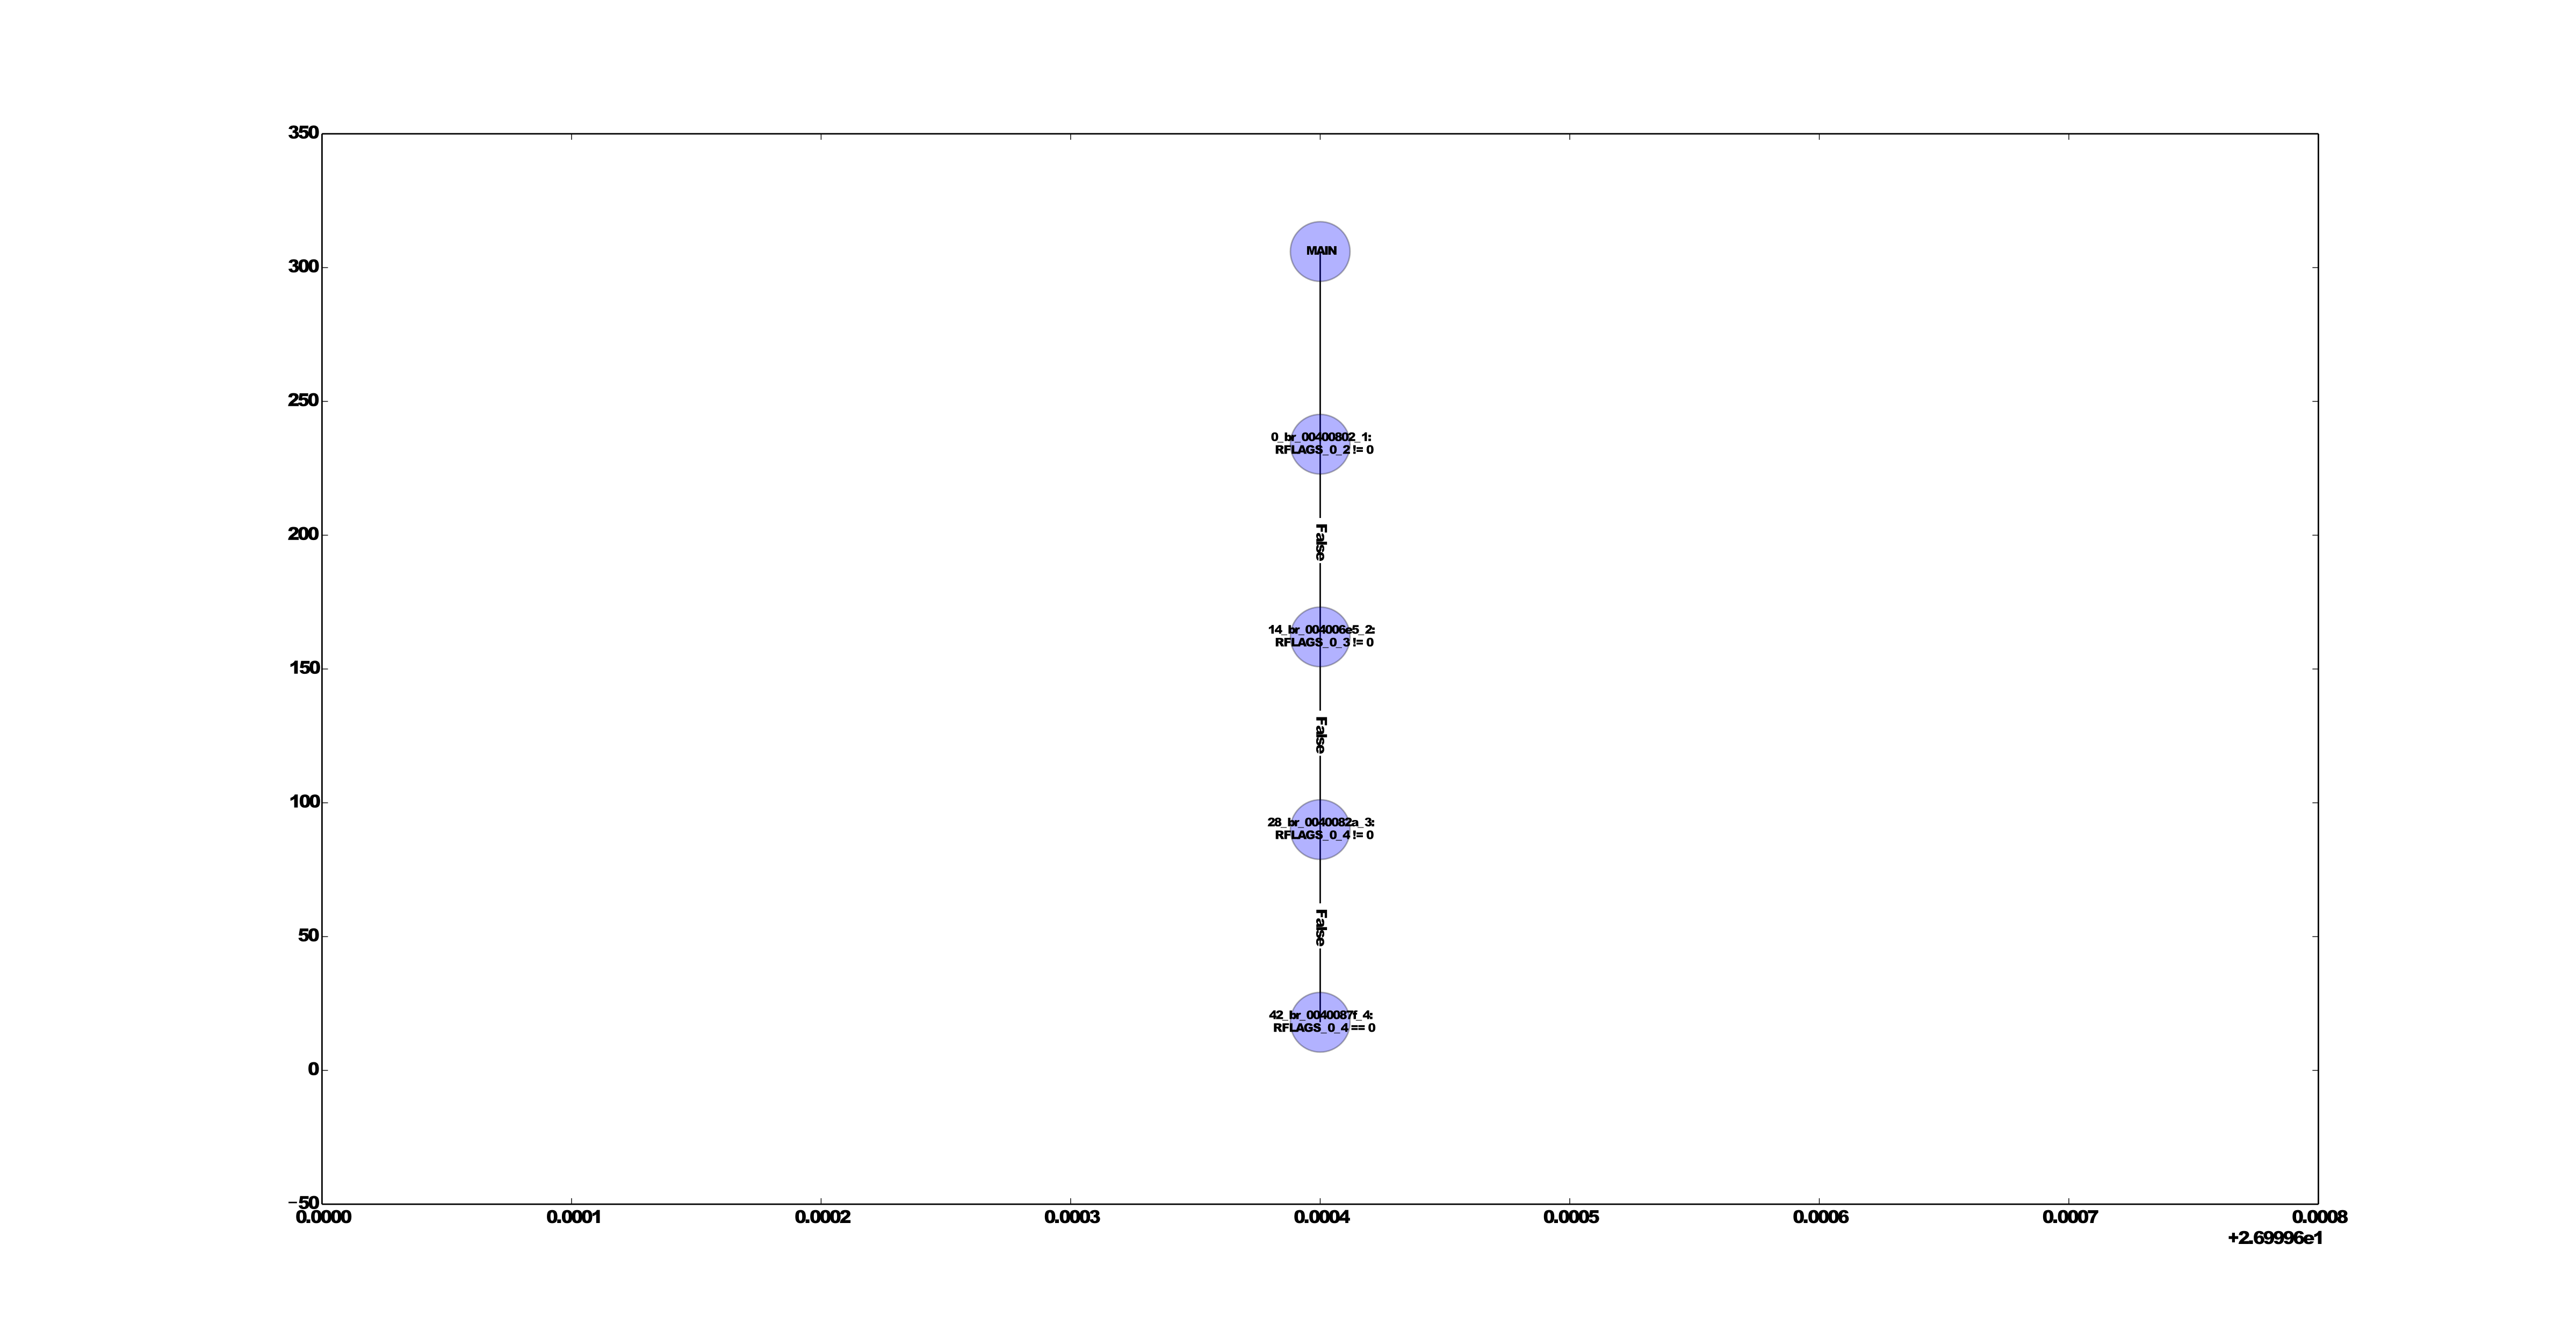
\includegraphics[width=0.45\textwidth]{graphs/1_0}
   &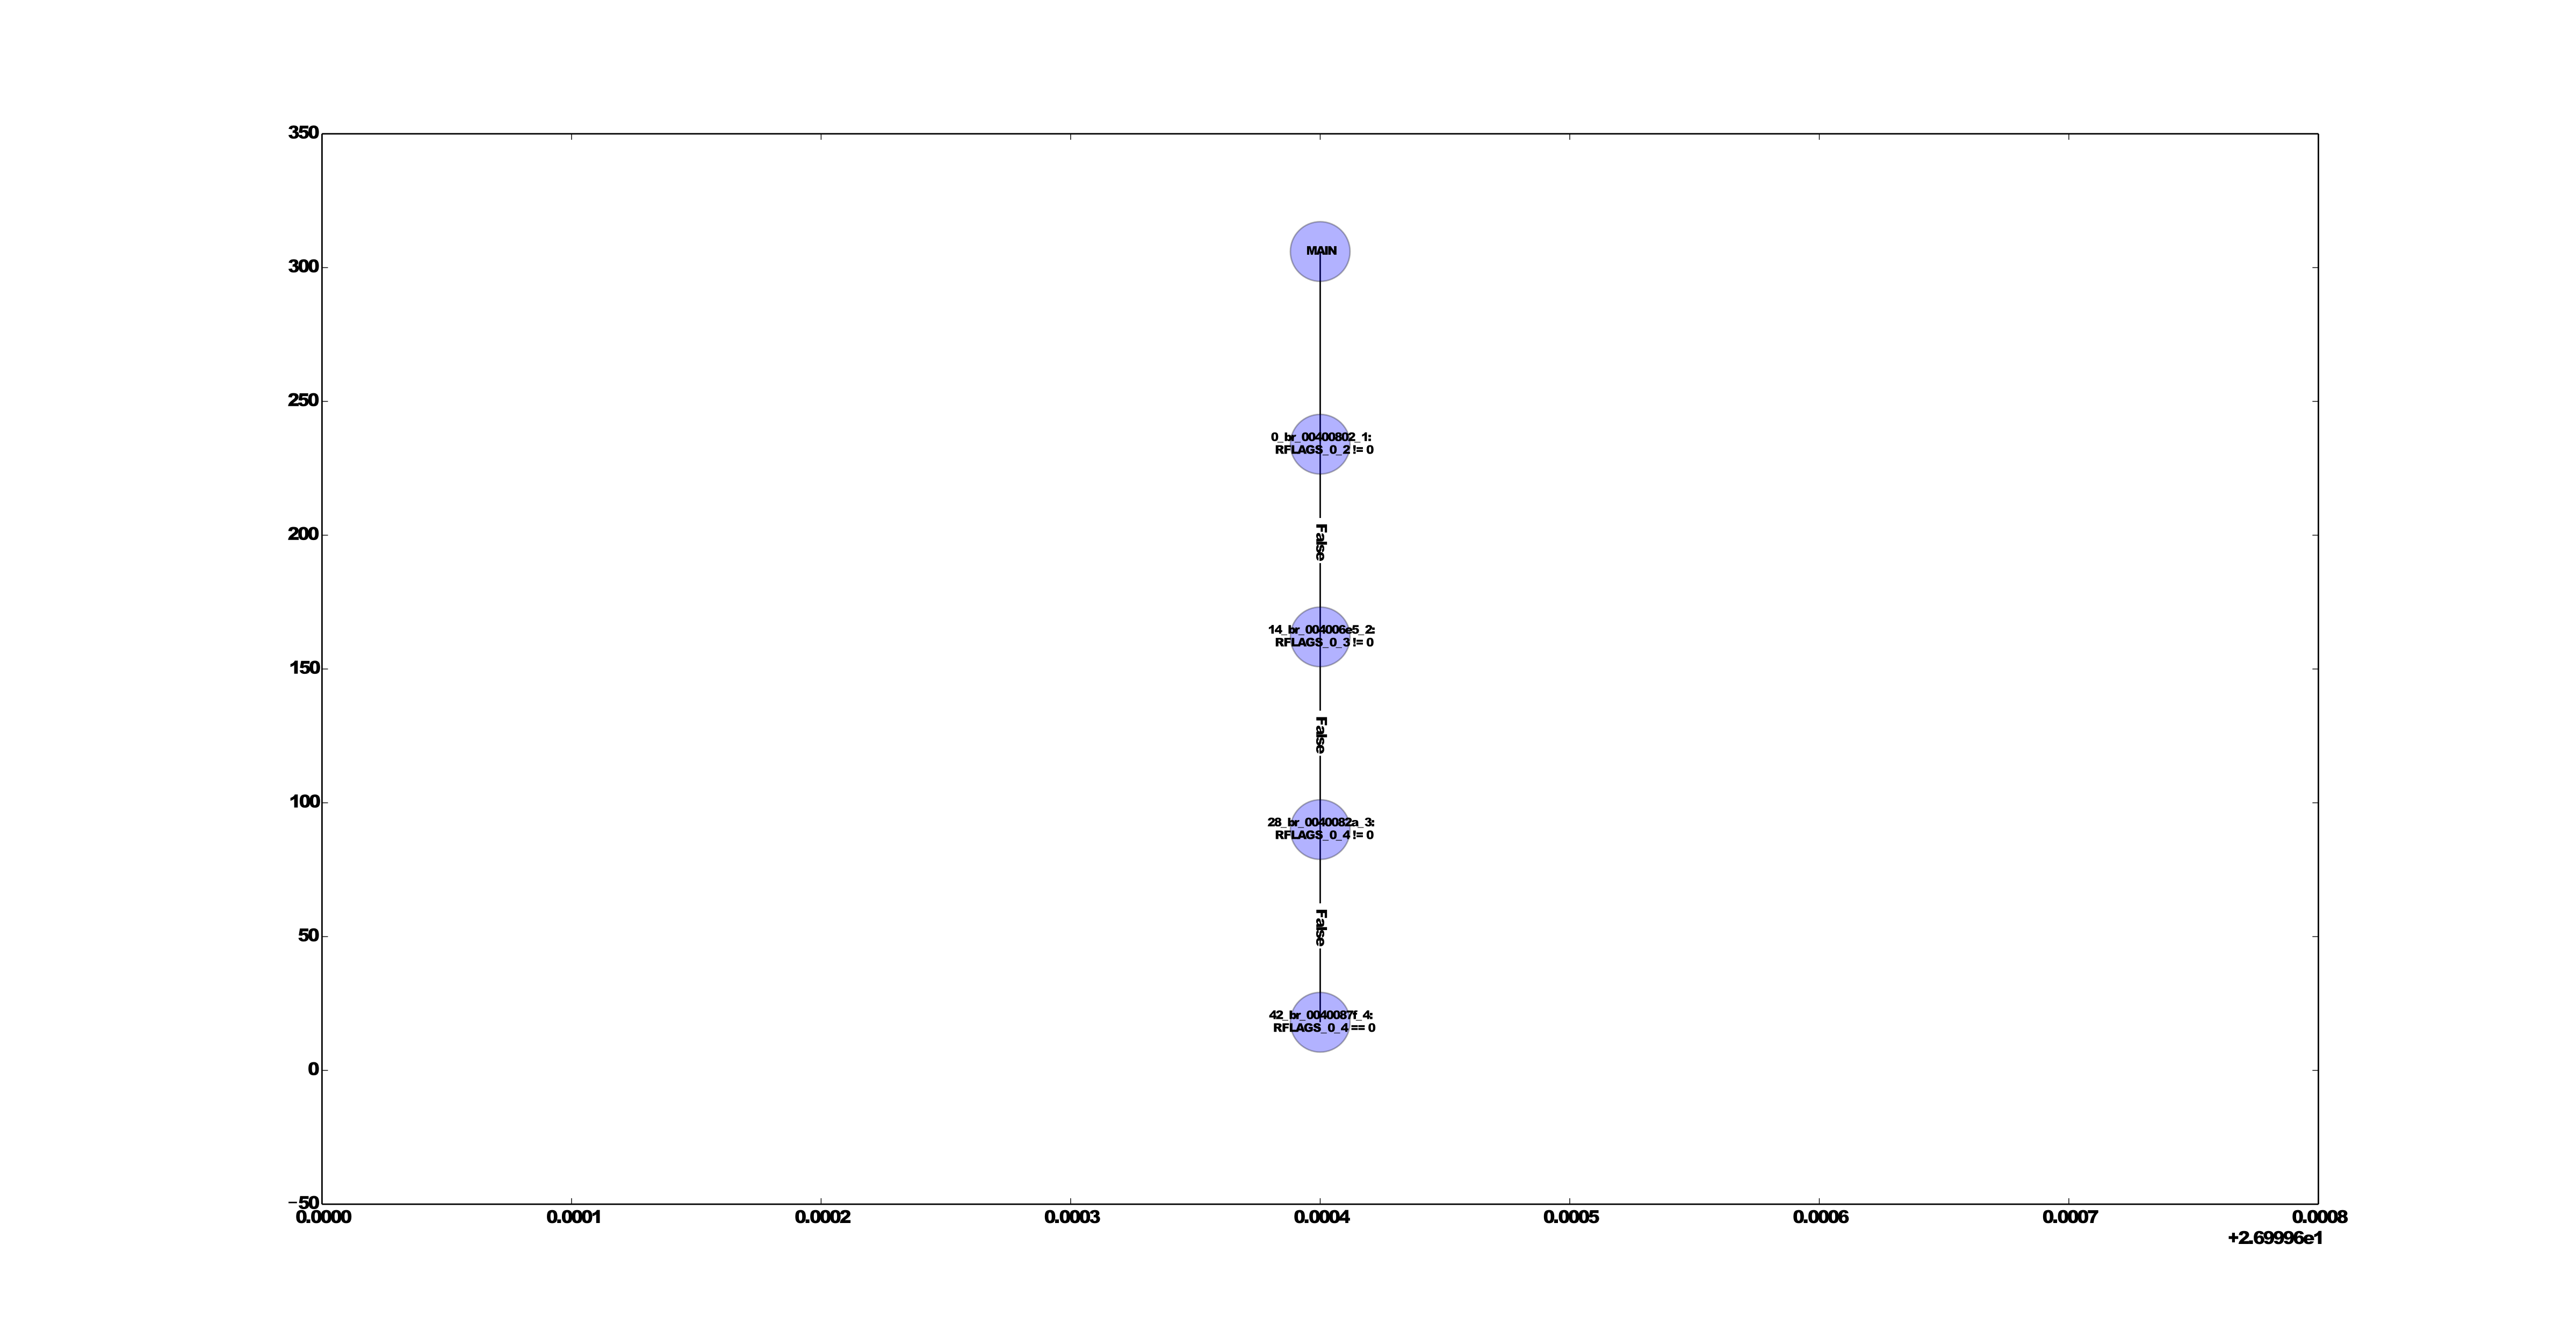
\includegraphics[width=0.45\textwidth]{graphs/1_1}\\\hline
   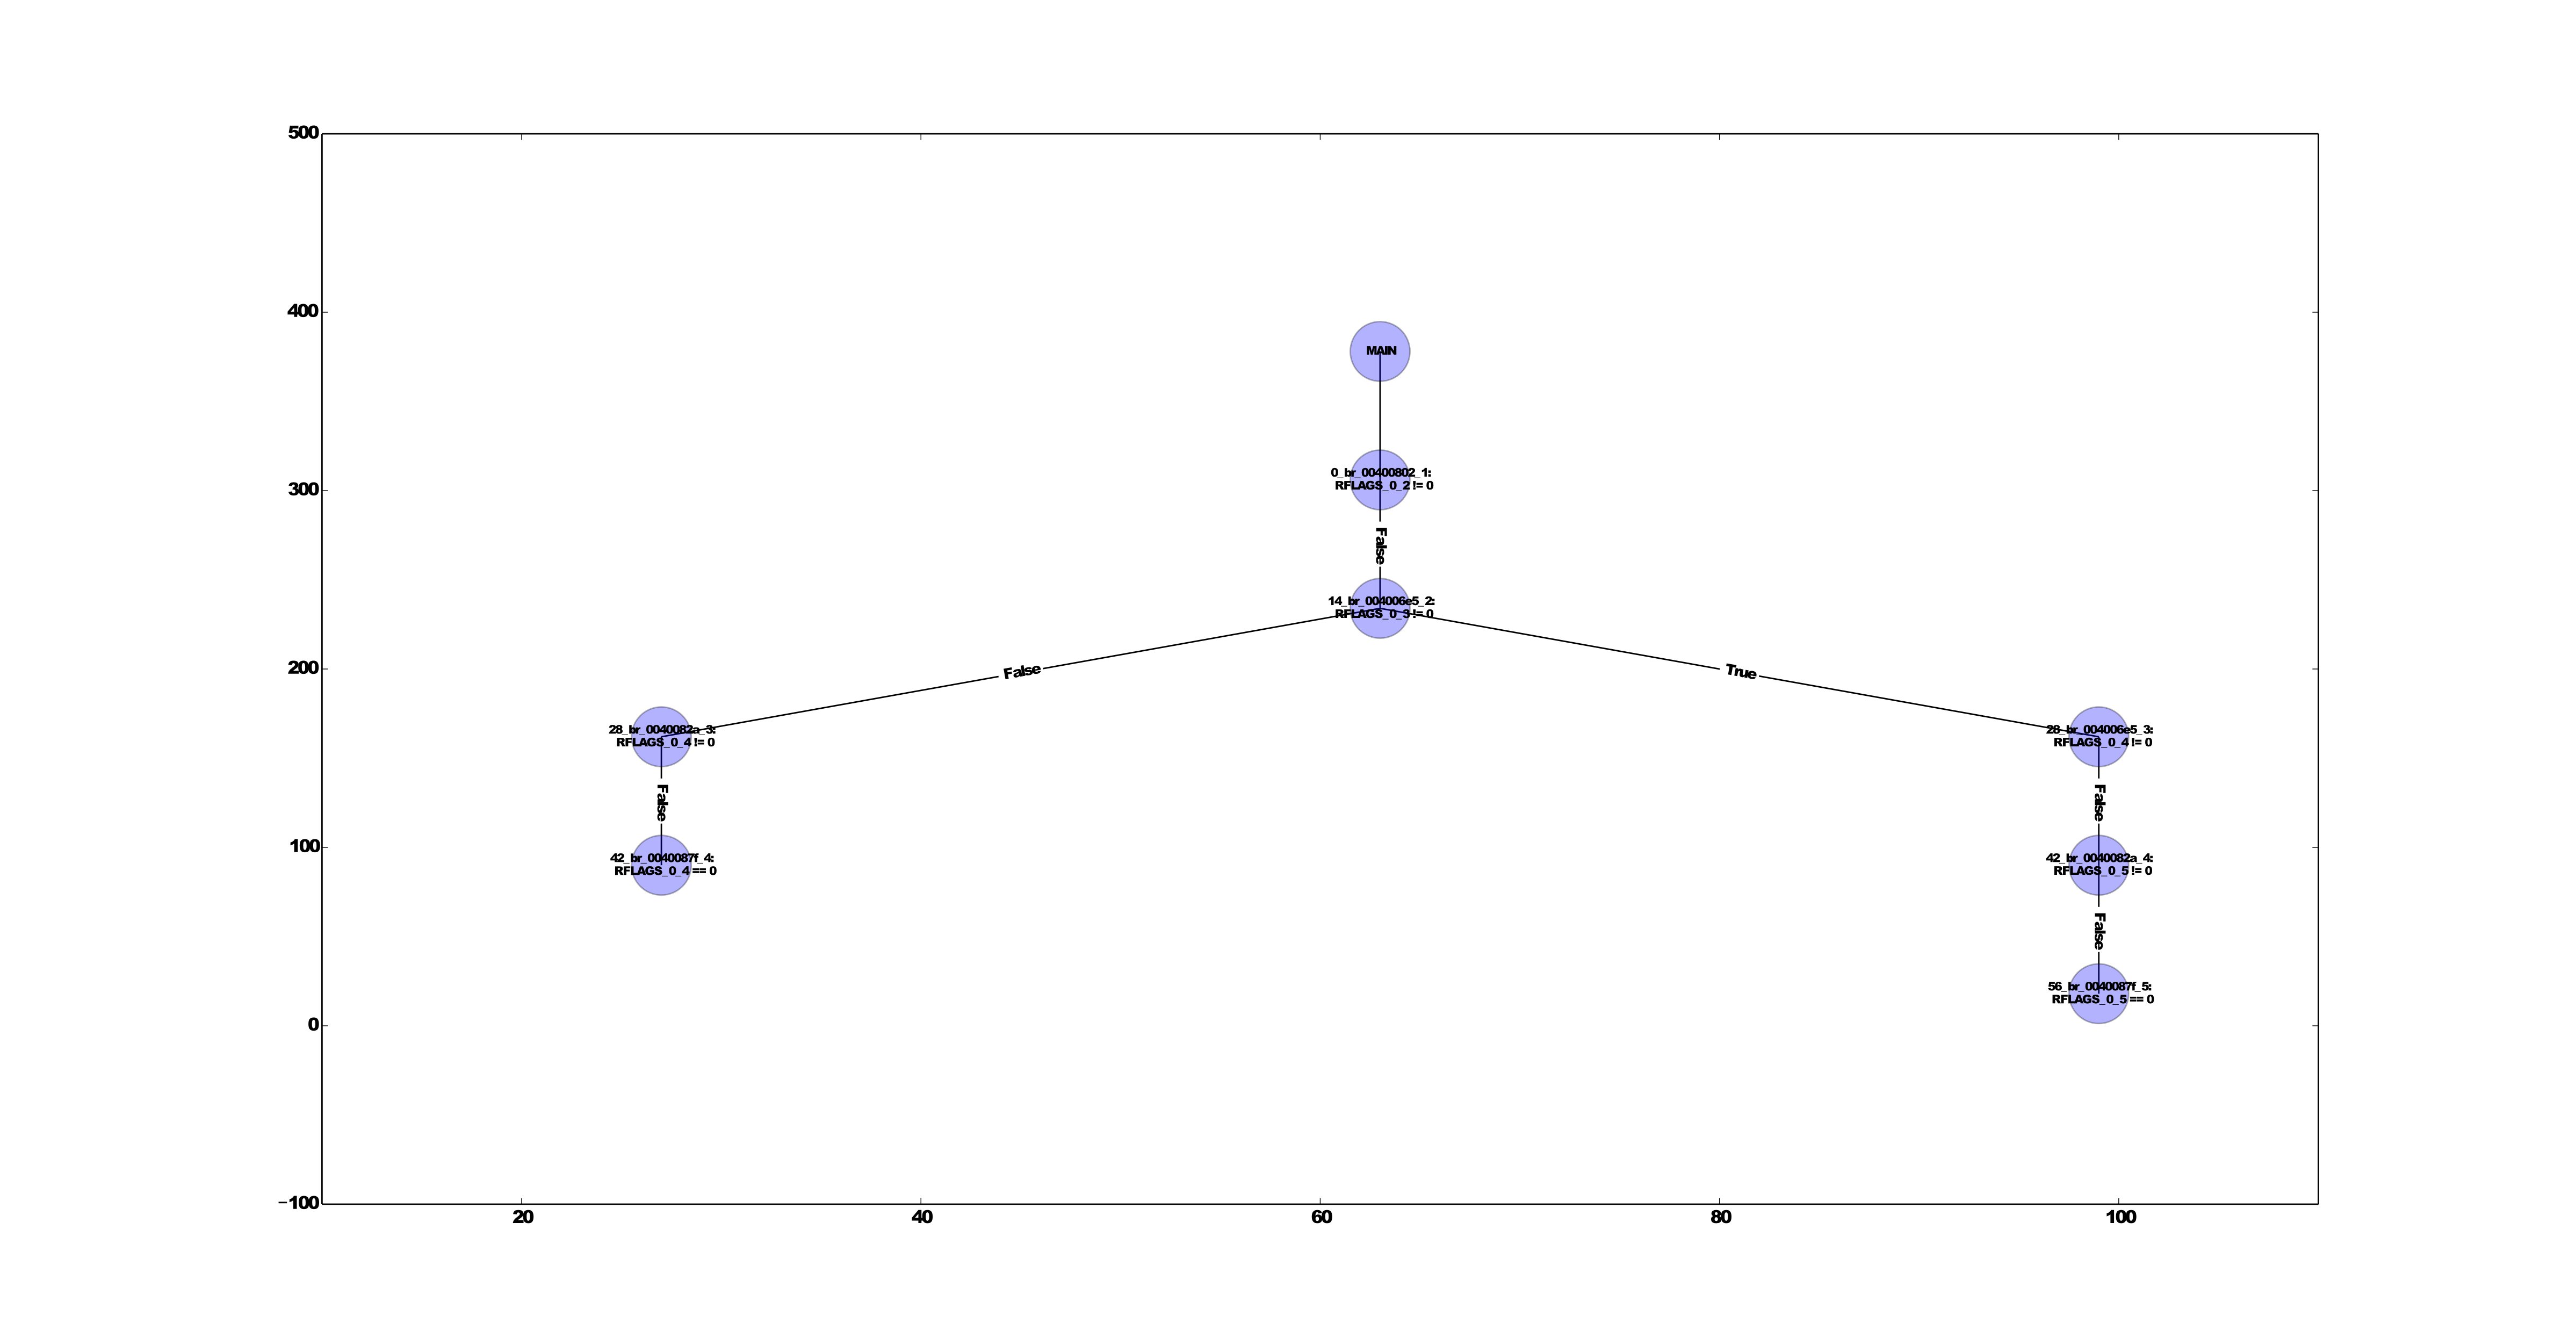
\includegraphics[width=0.45\textwidth]{graphs/1_2}
   &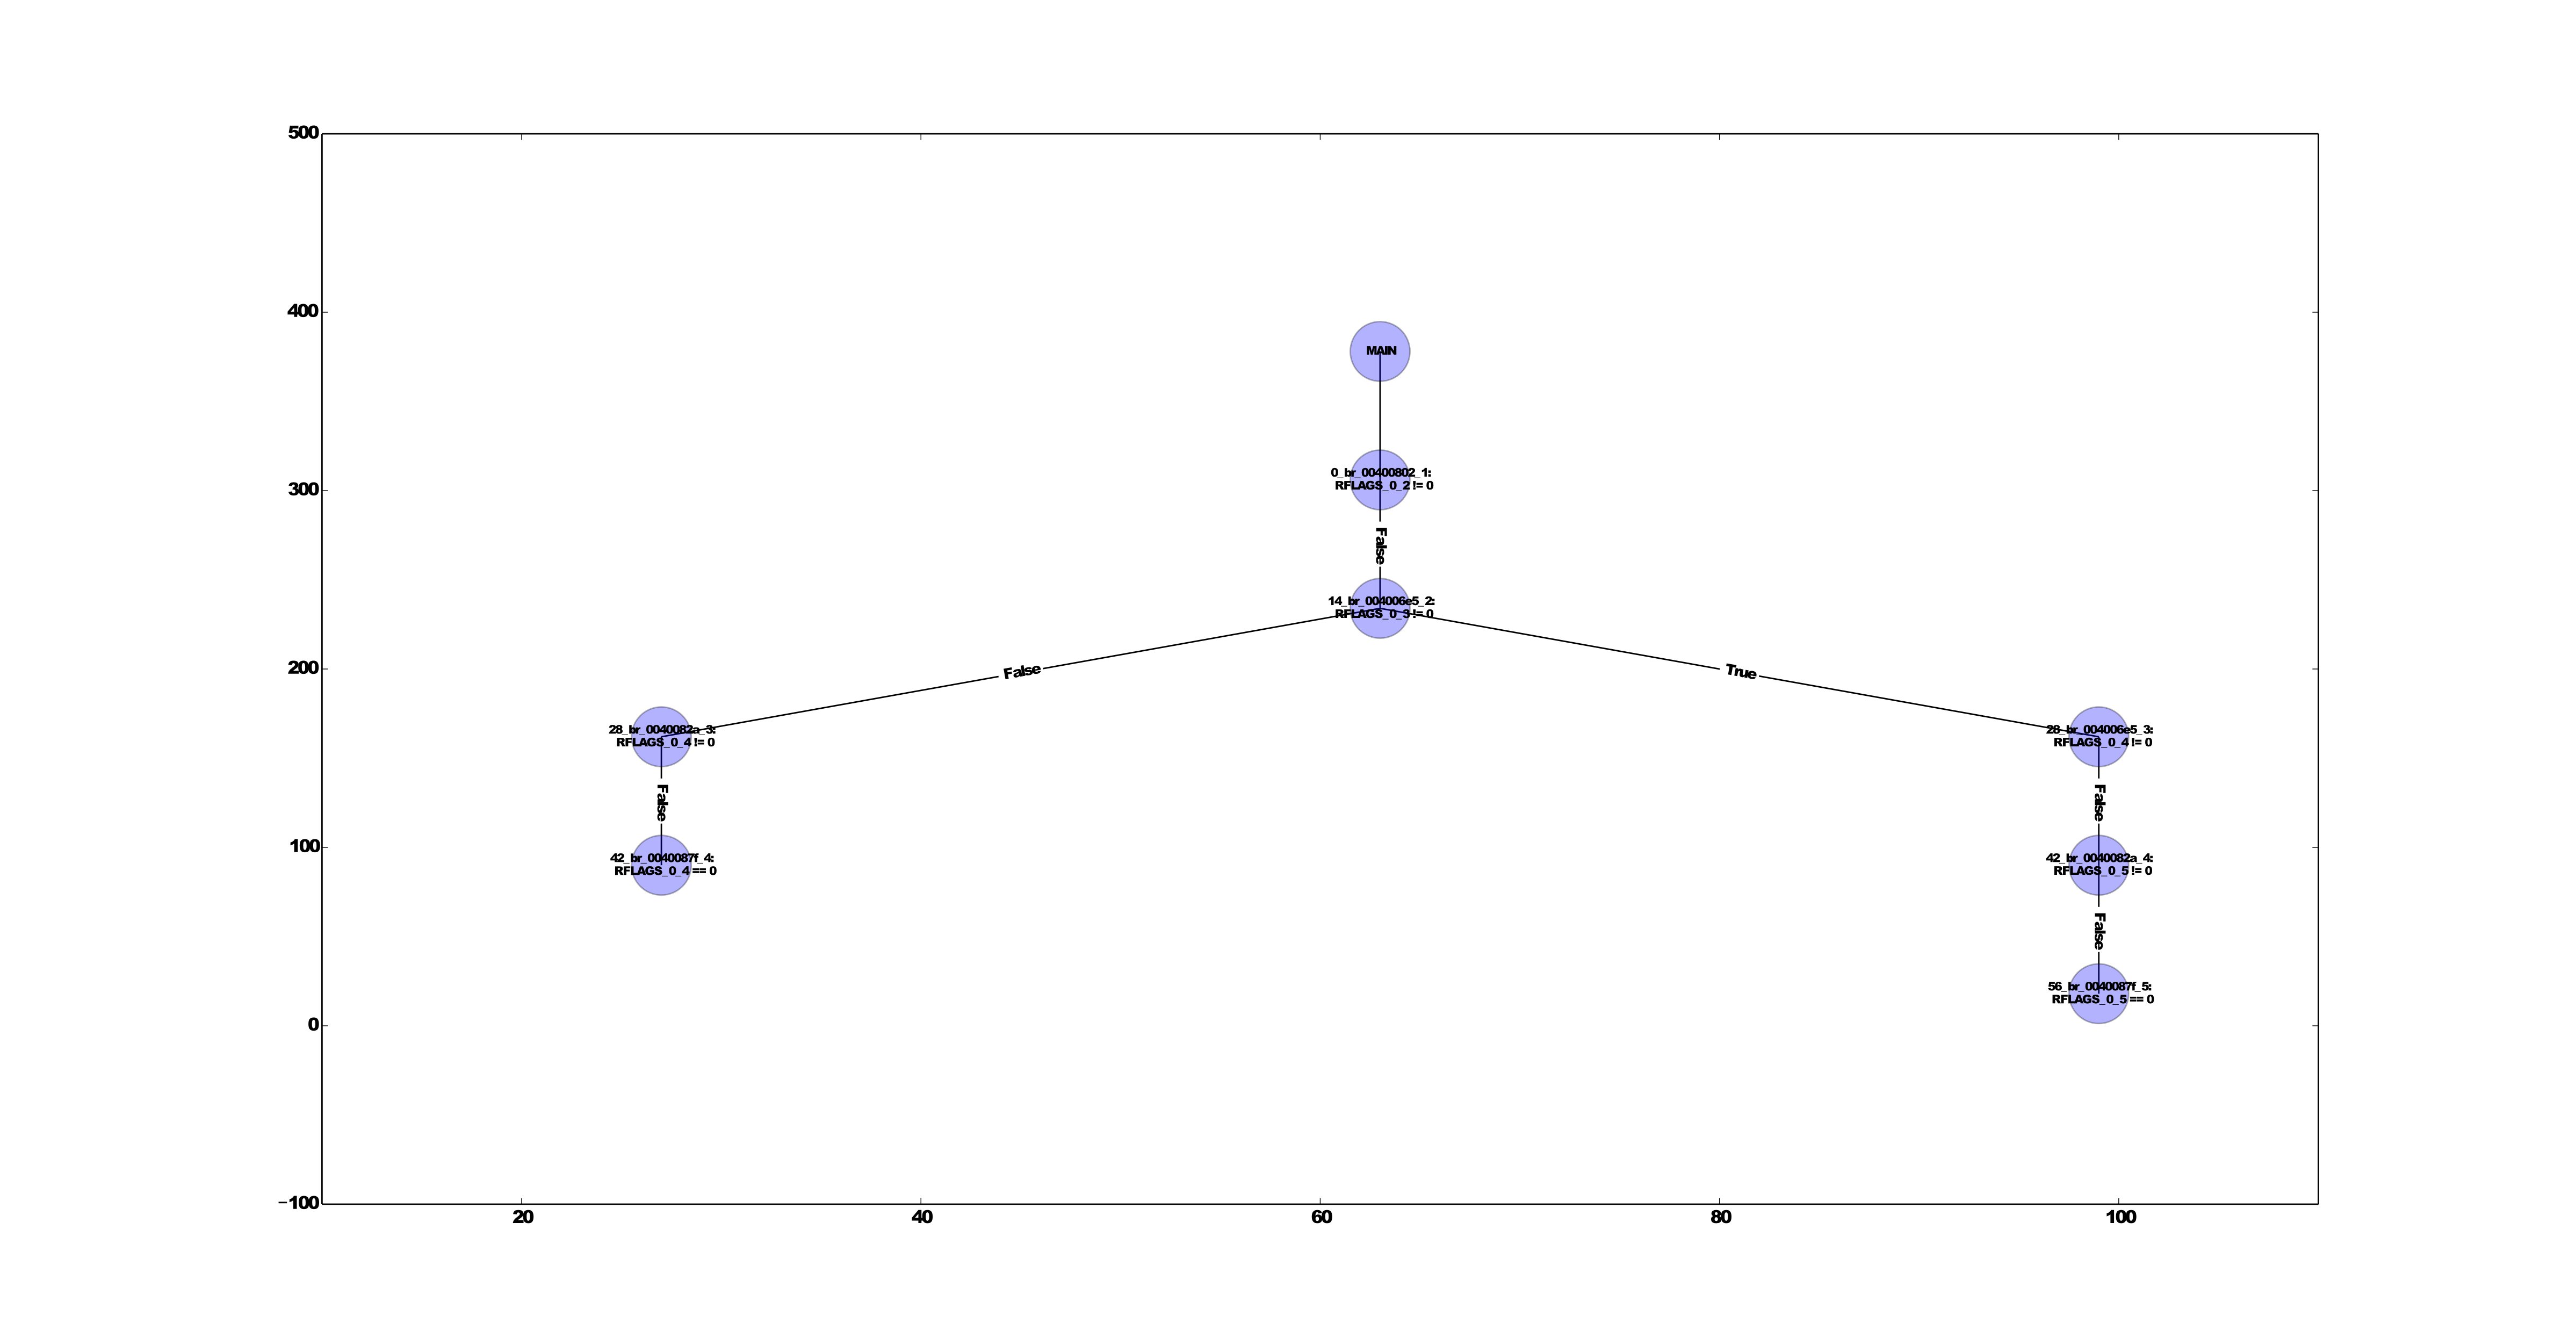
\includegraphics[width=0.45\textwidth]{graphs/1_3}\\\hline
   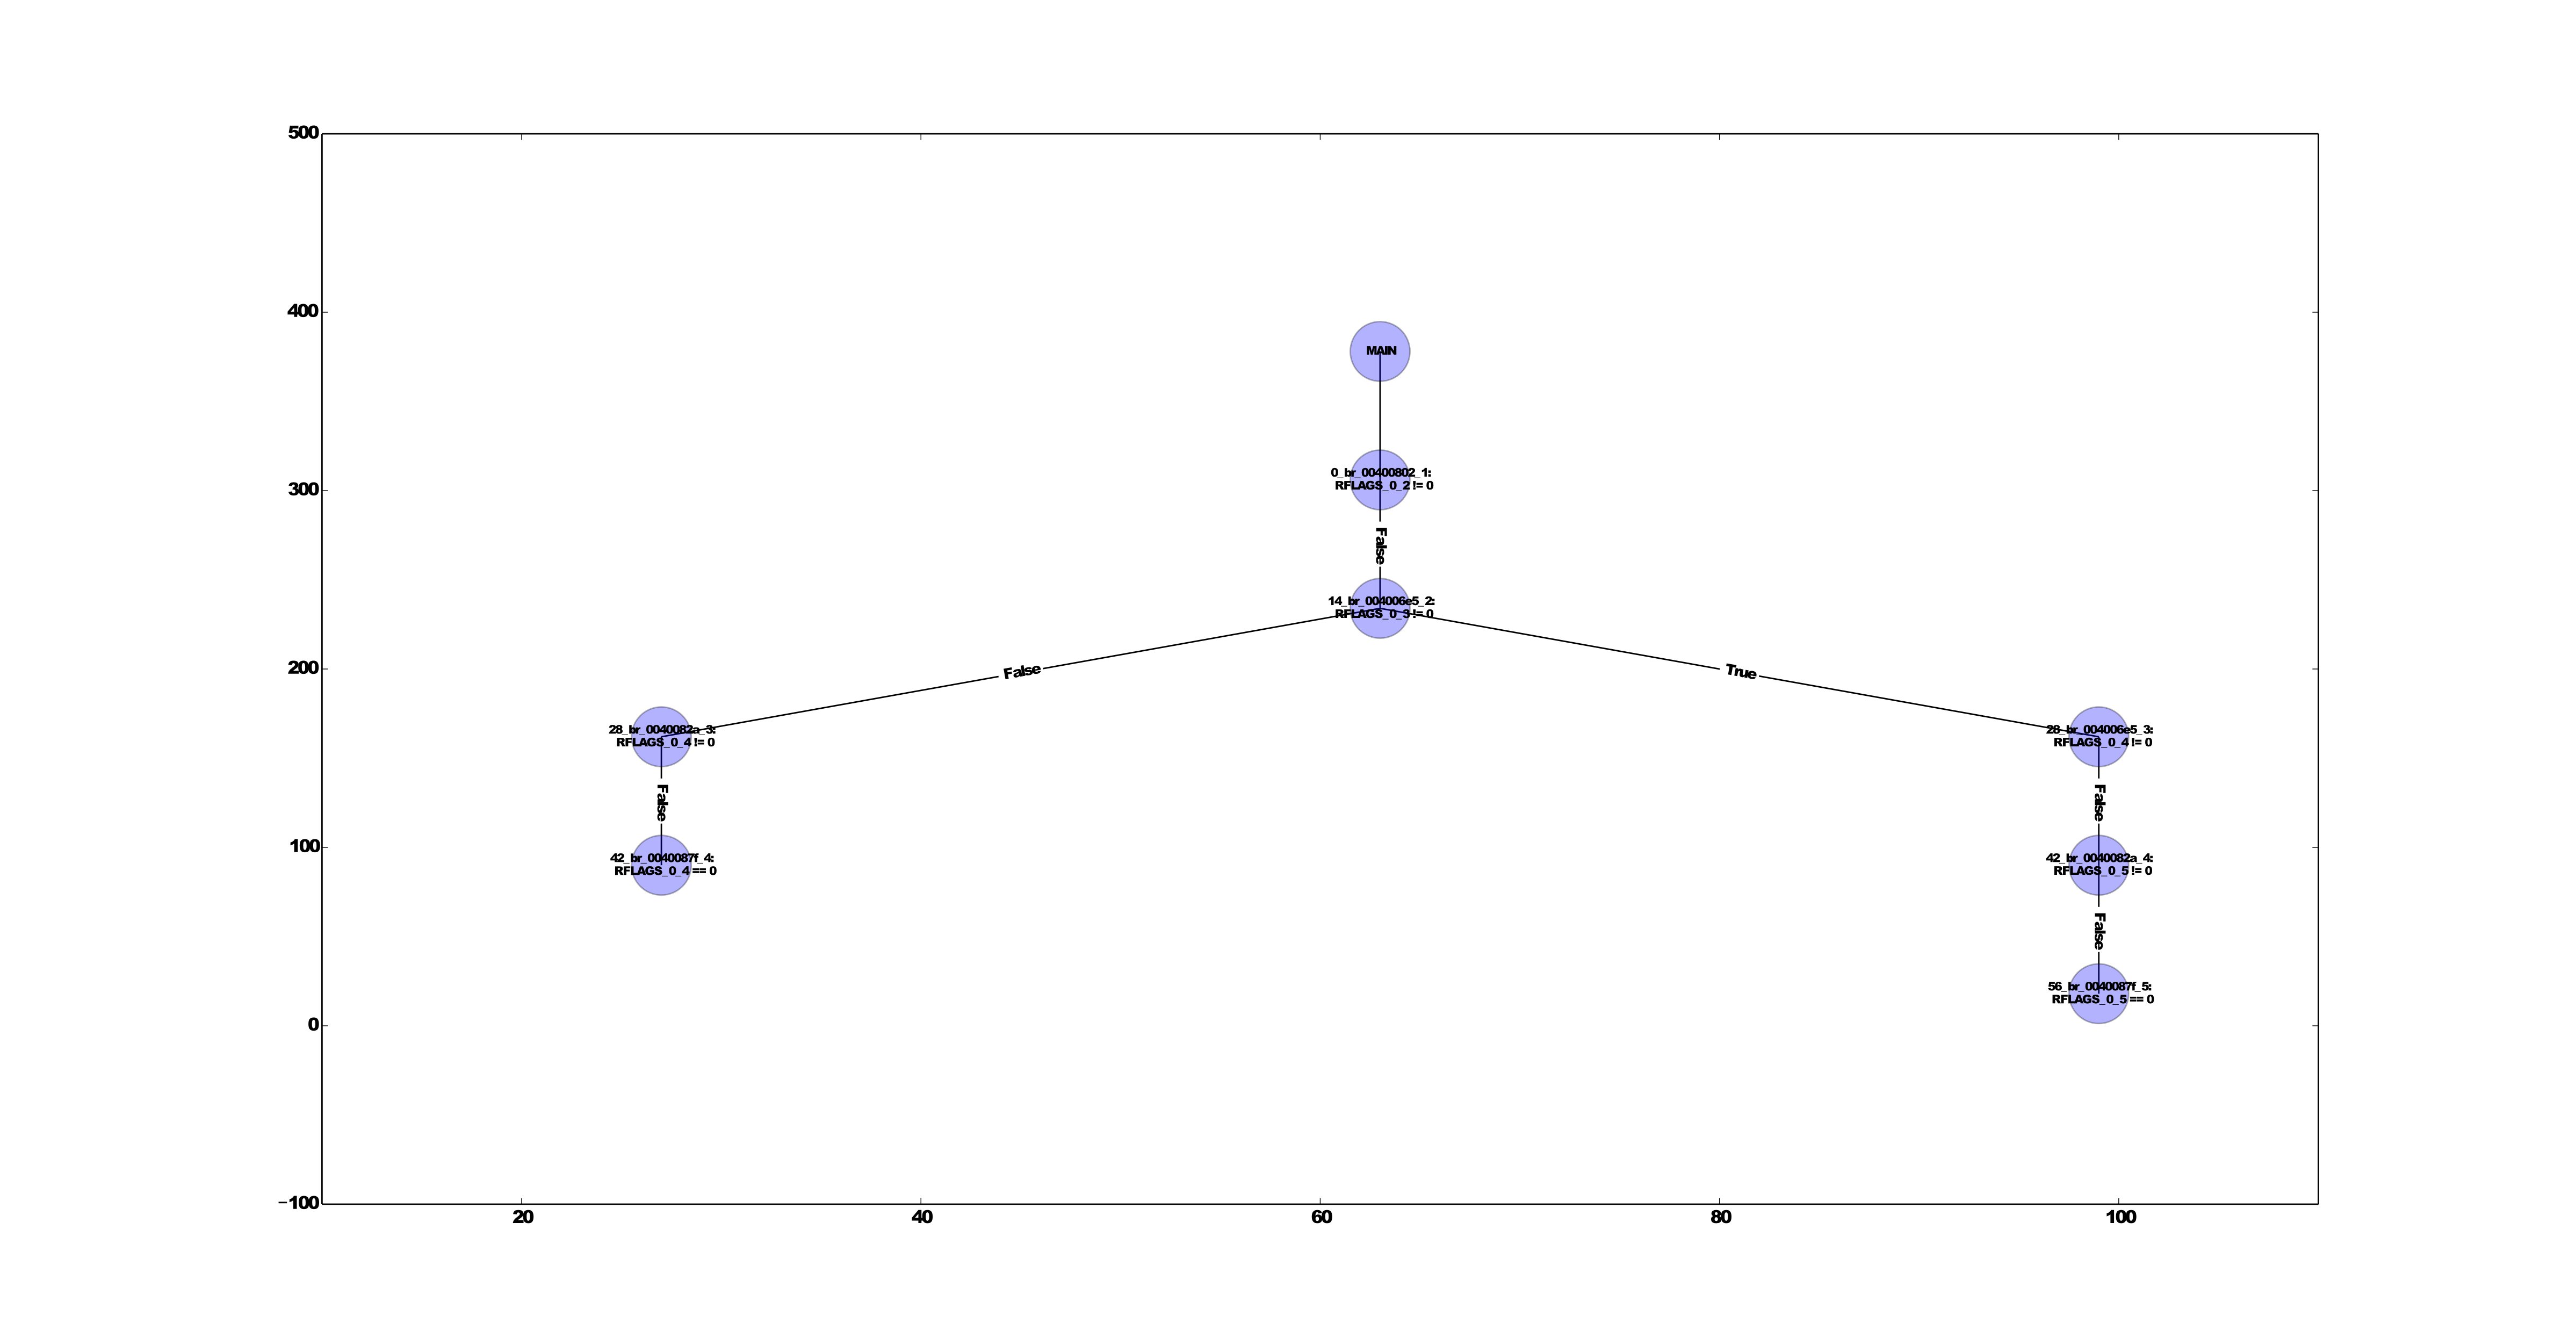
\includegraphics[width=0.45\textwidth]{graphs/1_4}
   &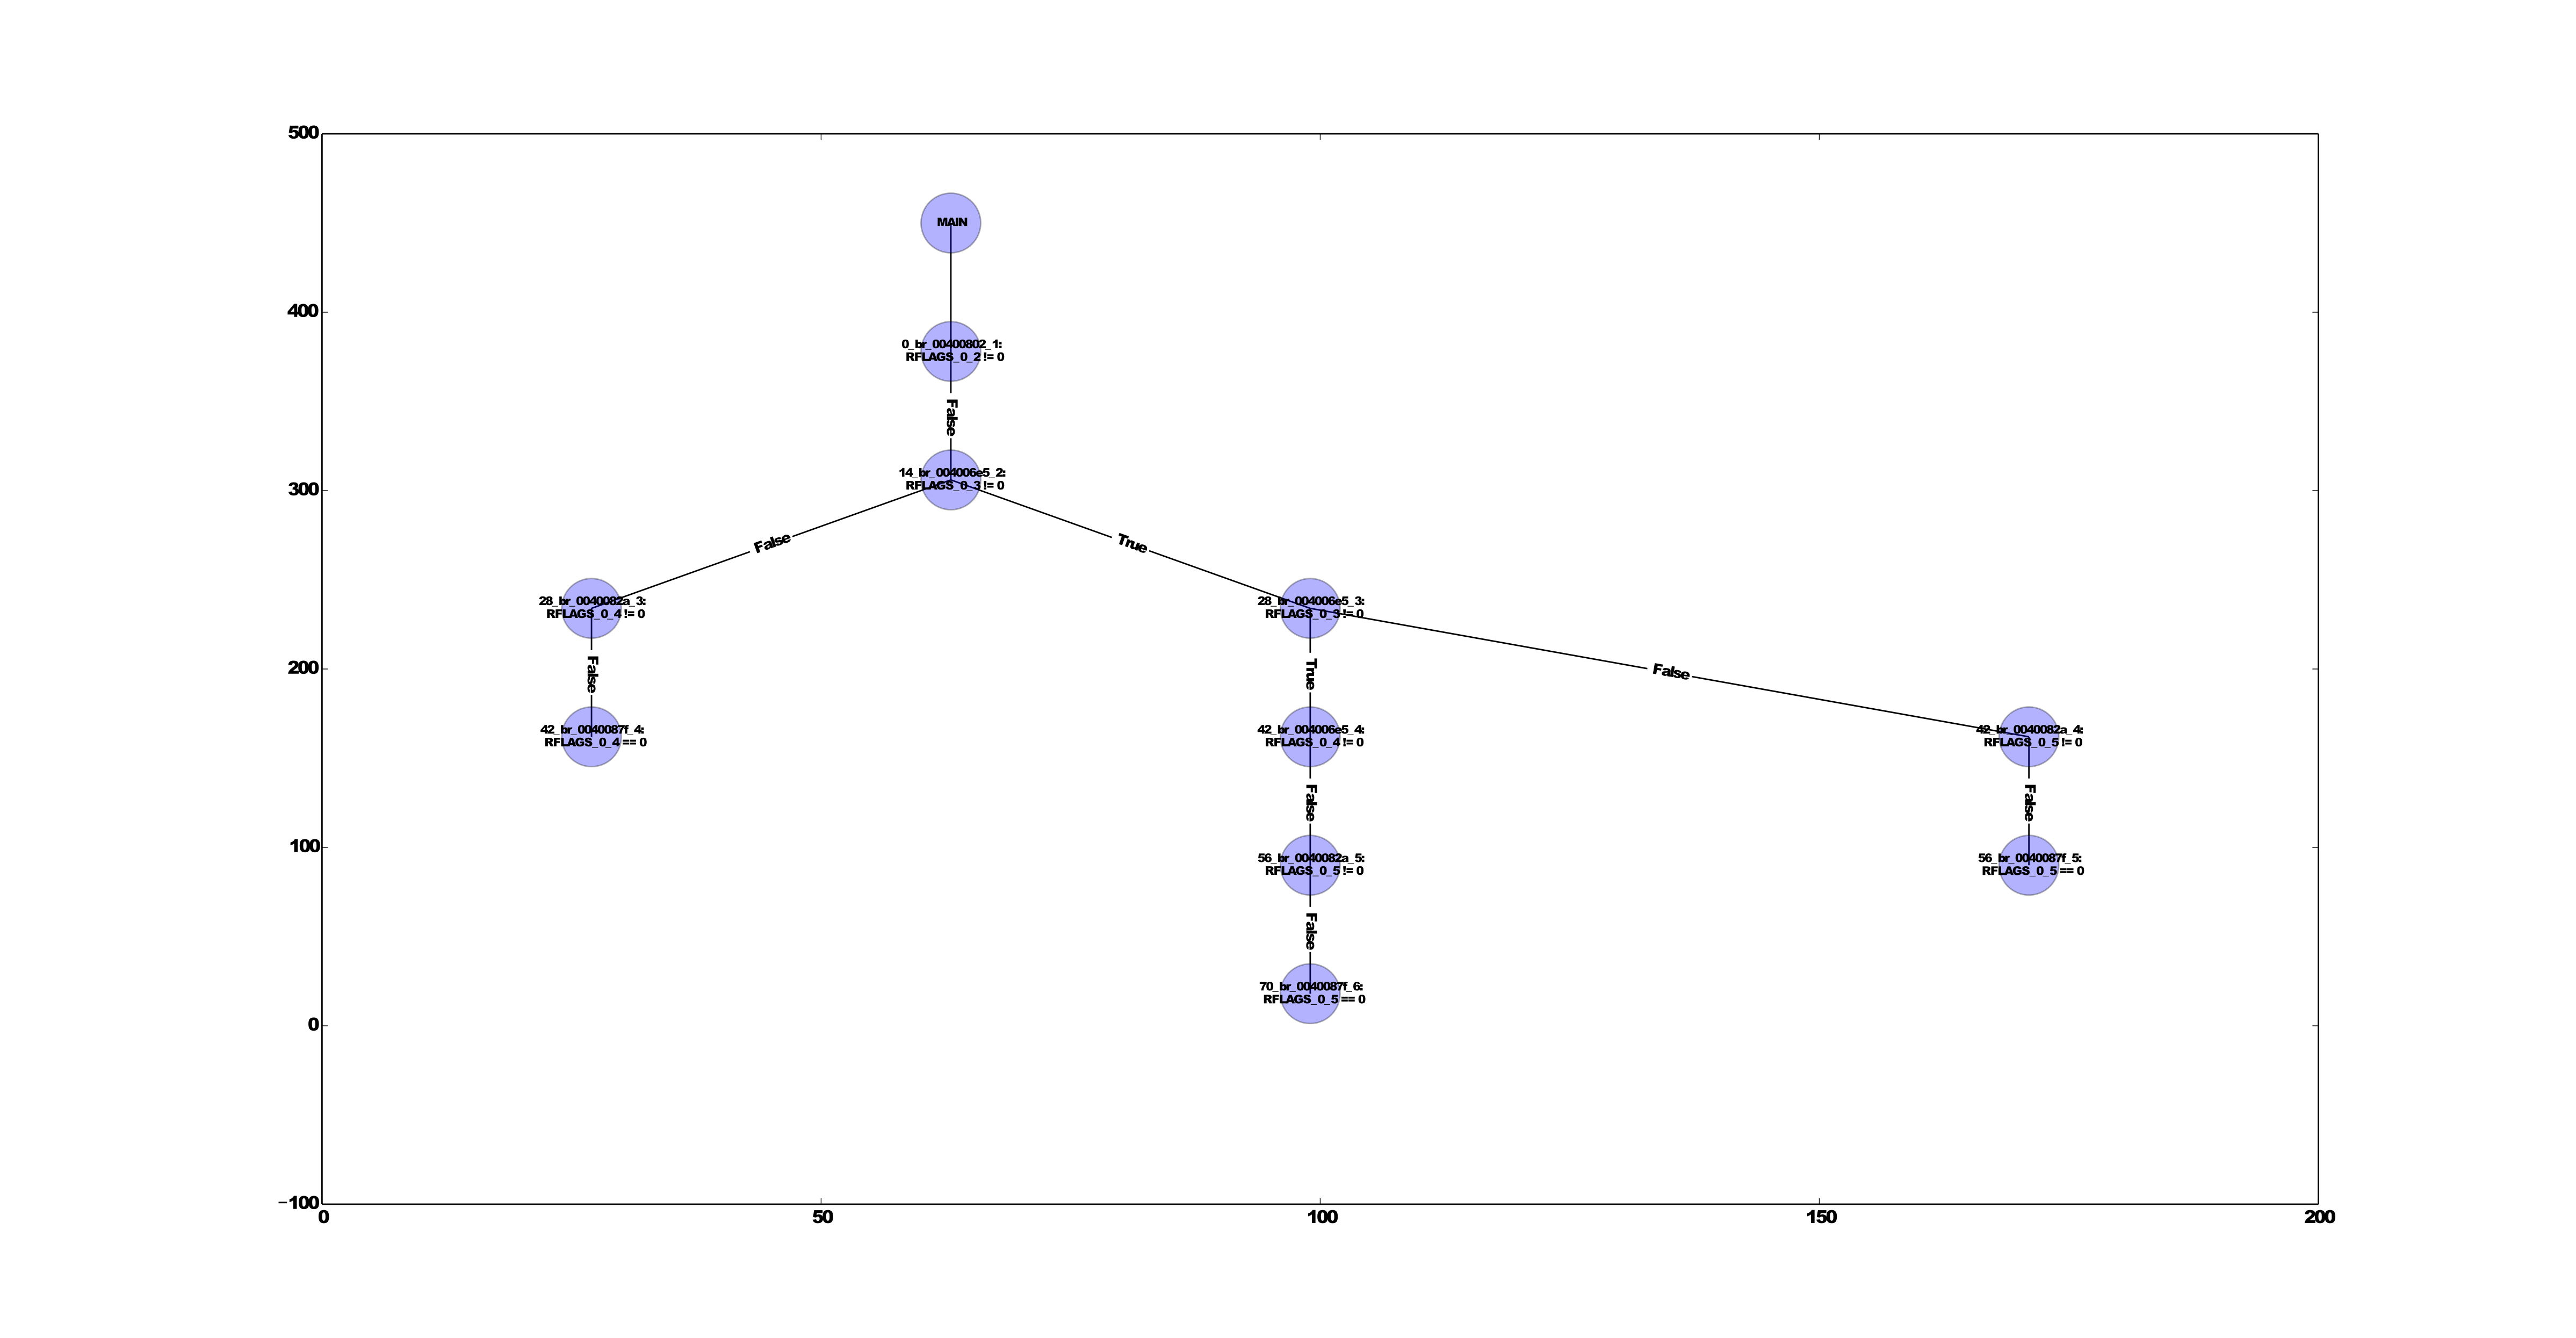
\includegraphics[width=0.45\textwidth]{graphs/1_5}\\\hline
   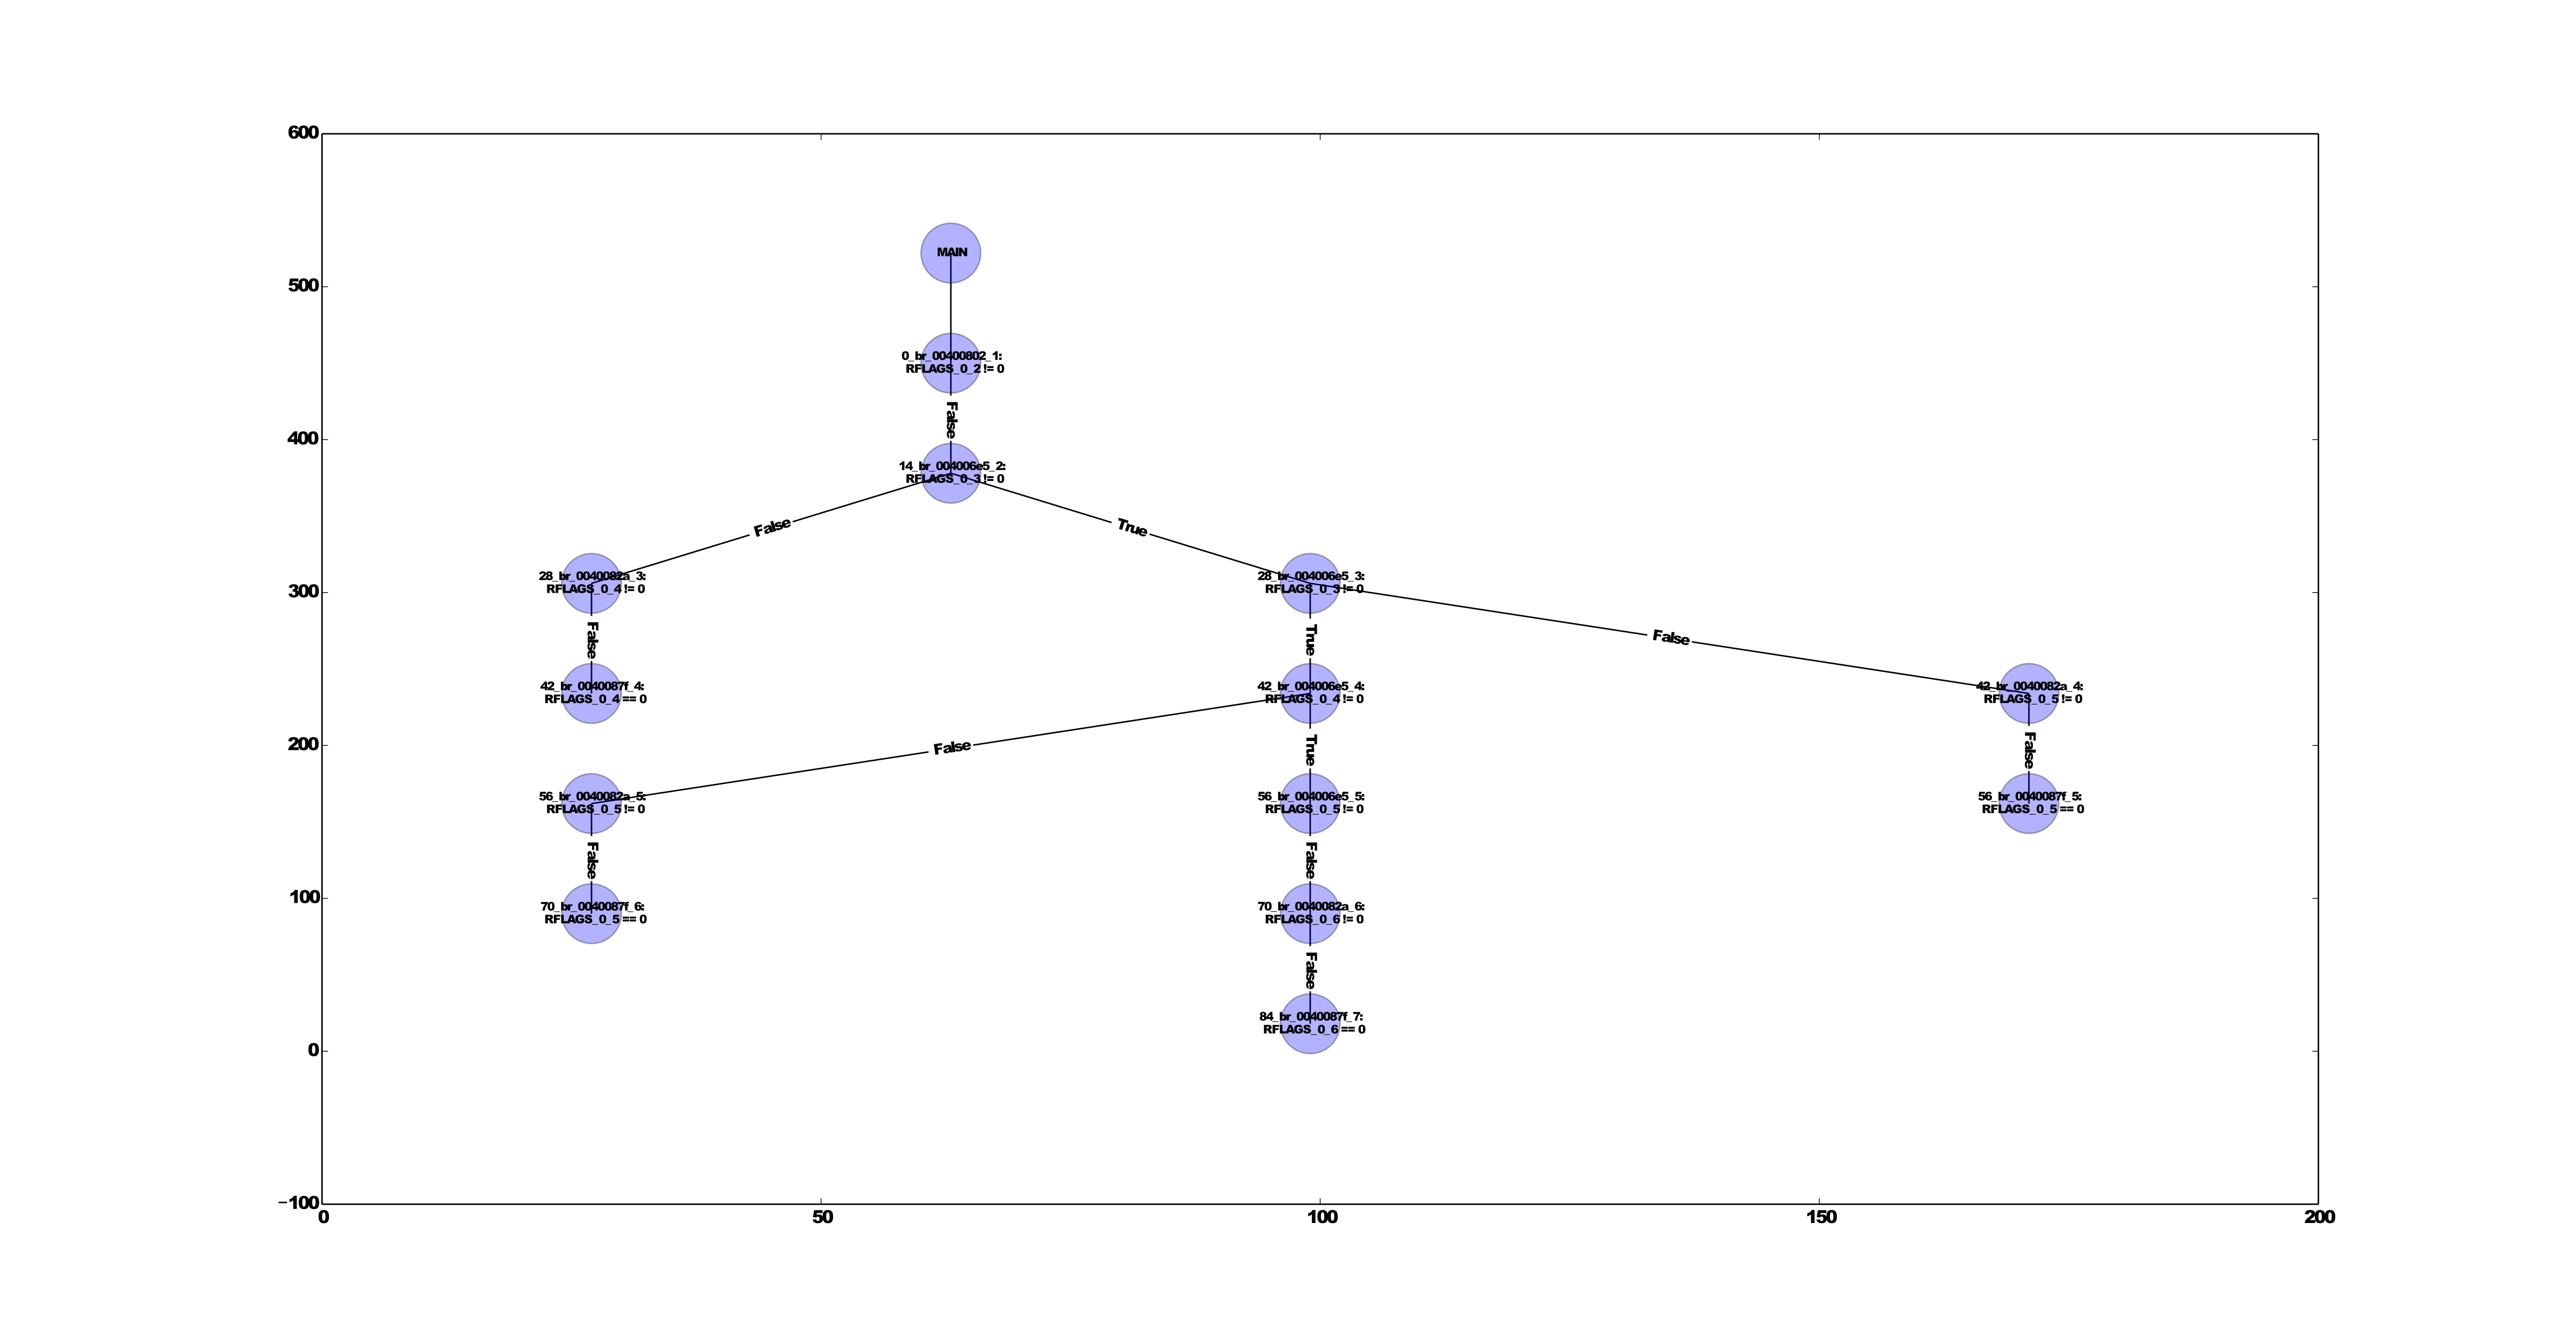
\includegraphics[width=0.45\textwidth]{graphs/1_6}
   &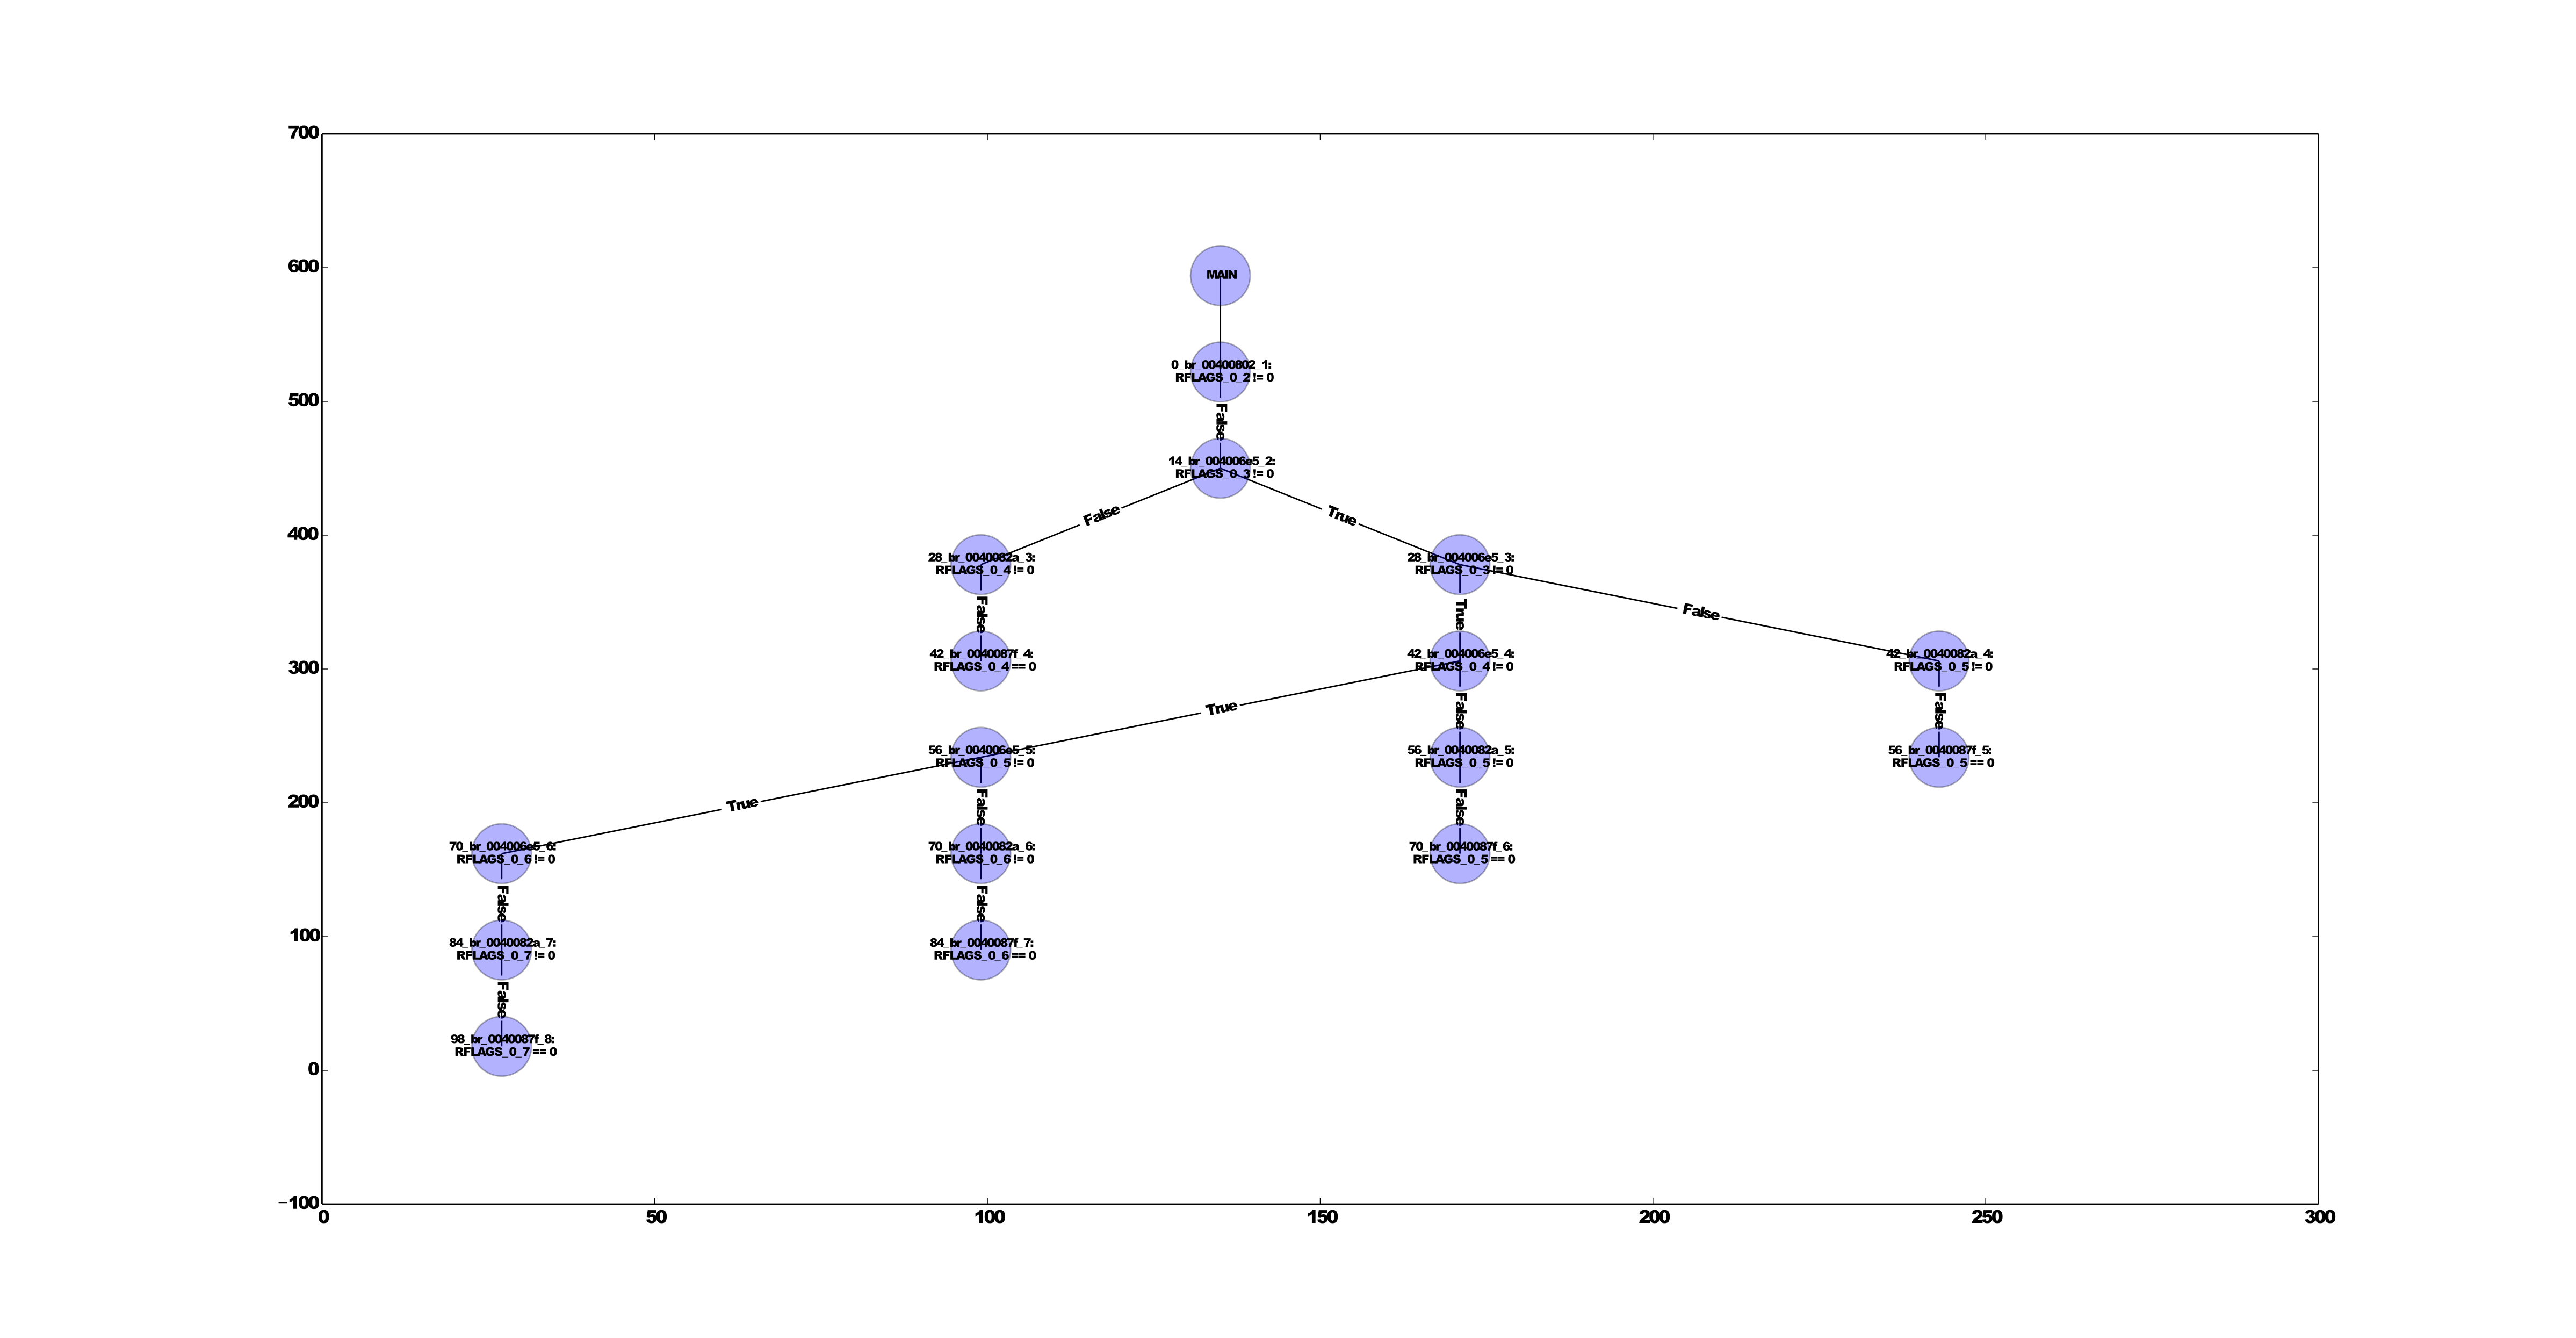
\includegraphics[width=0.45\textwidth]{graphs/1_7}\\\hline
 \end{tabular}
 \caption{Example Execution Graphs for test1}
 \label{figure:examplegraphs}
\end{figure}

\begin{figure}[ht]
 \centering
 \begin{tabular}{| c | c |}
   \hline
   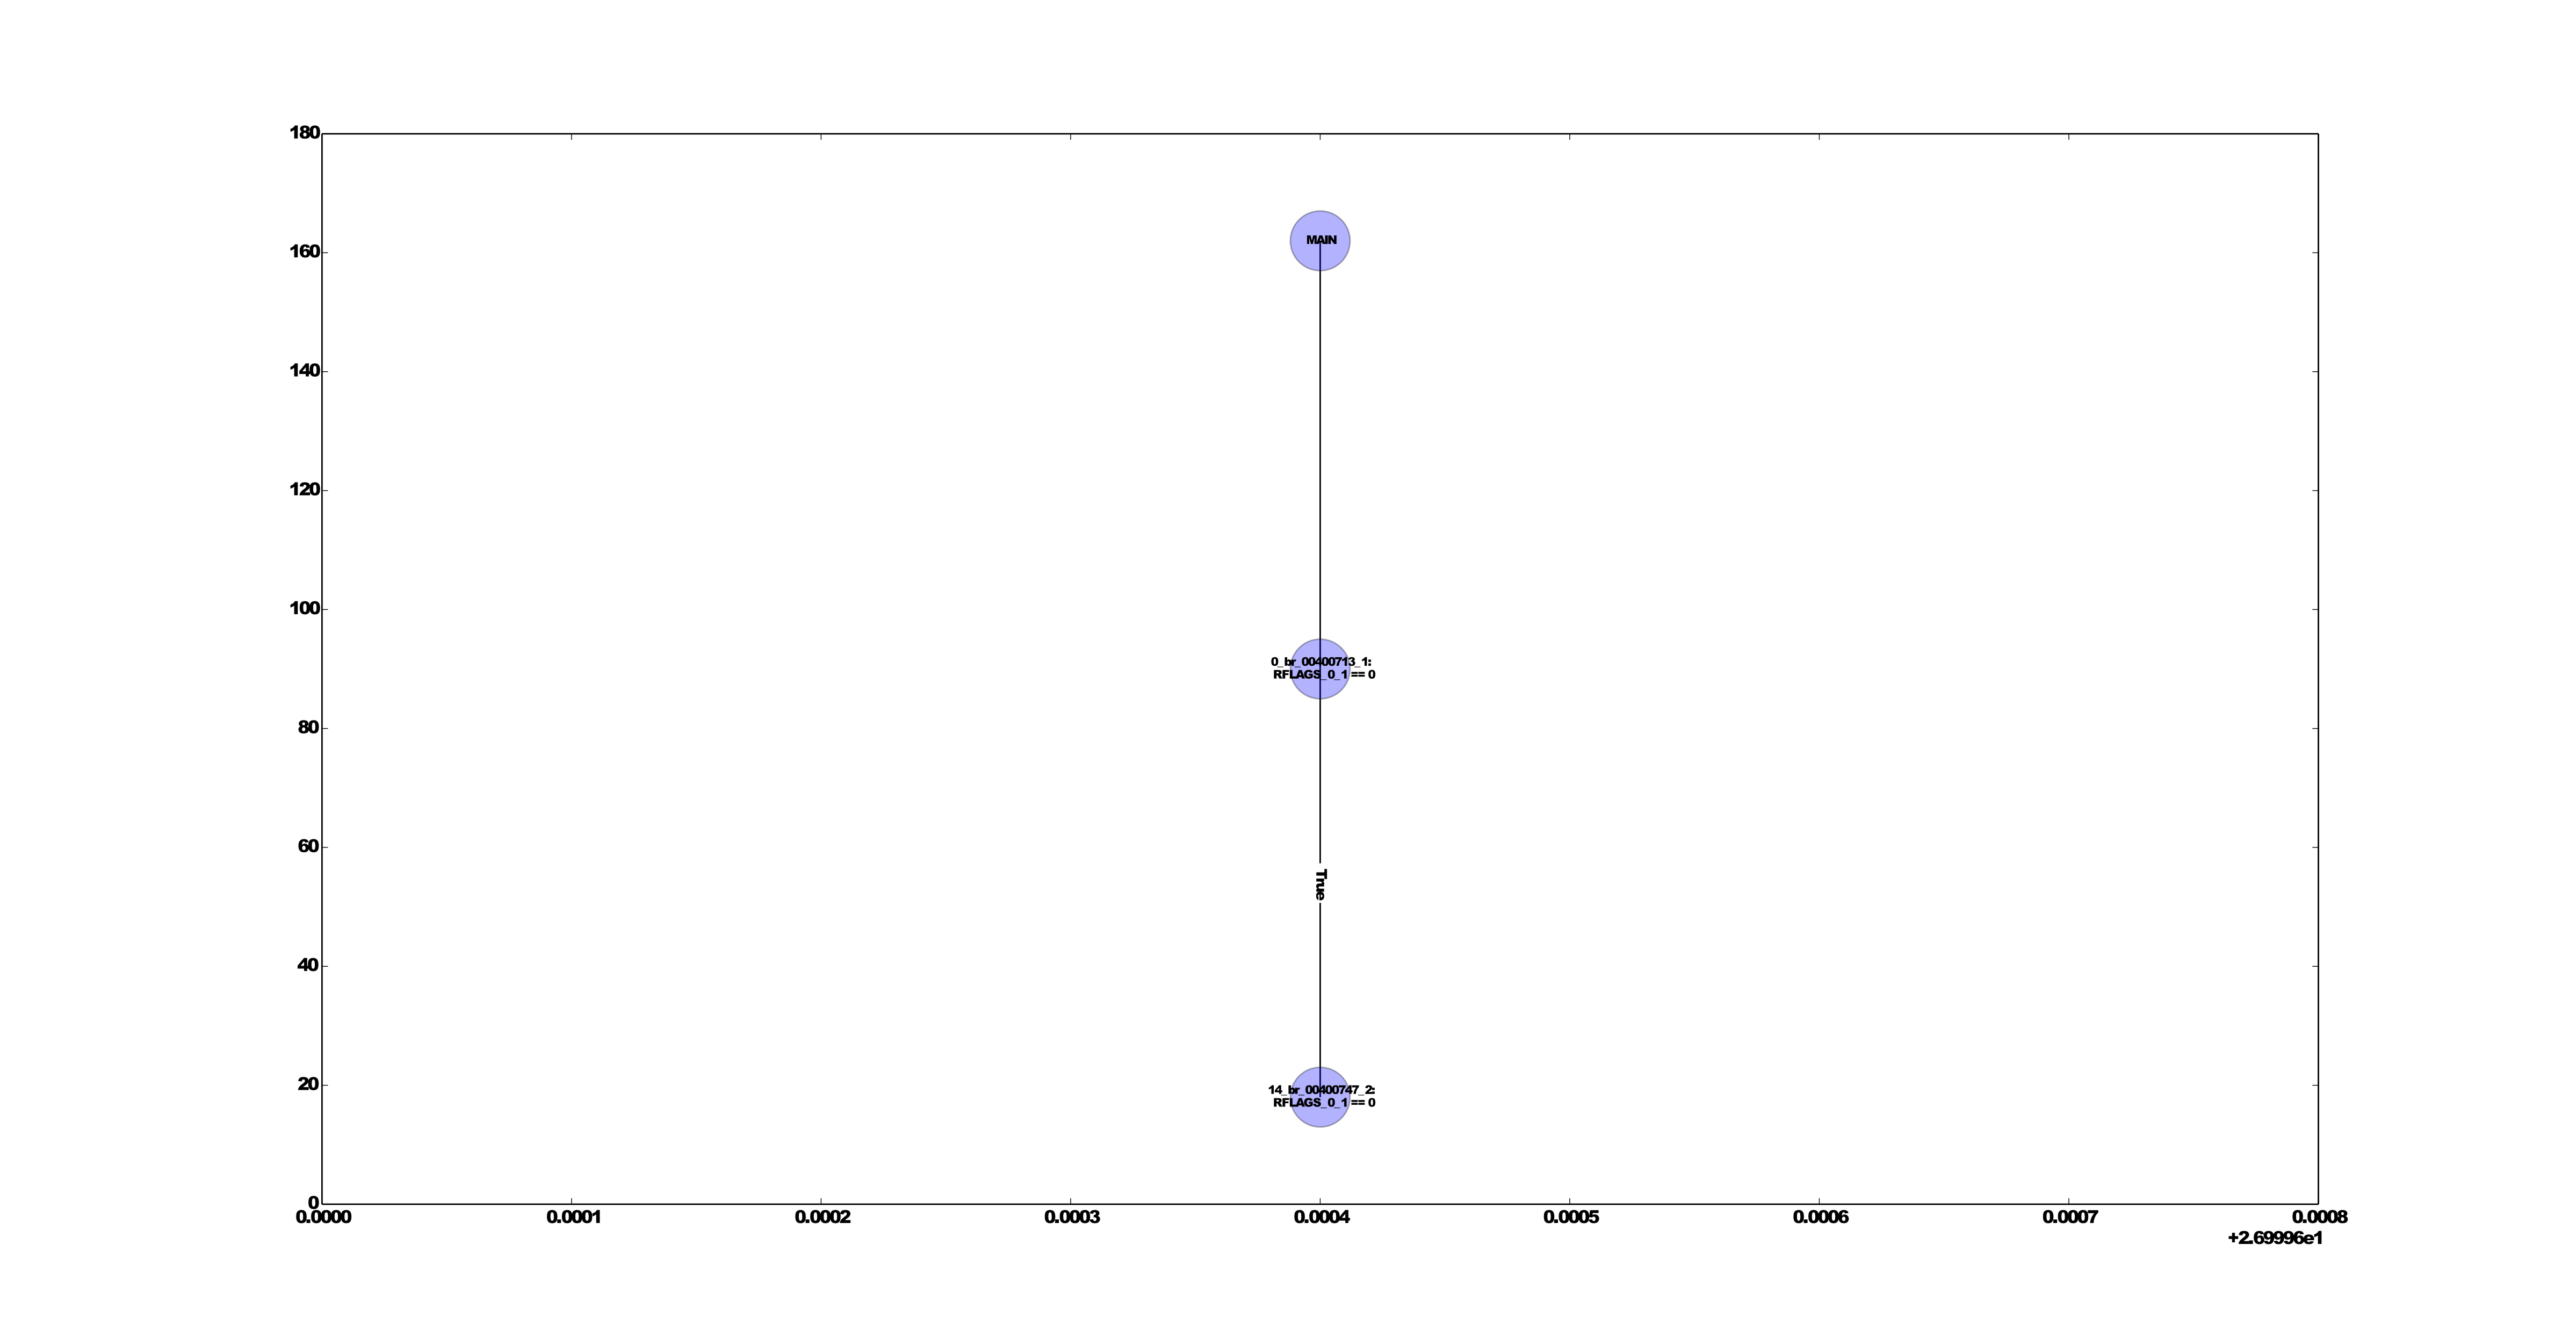
\includegraphics[width=0.45\textwidth]{graphs/2_0}
   &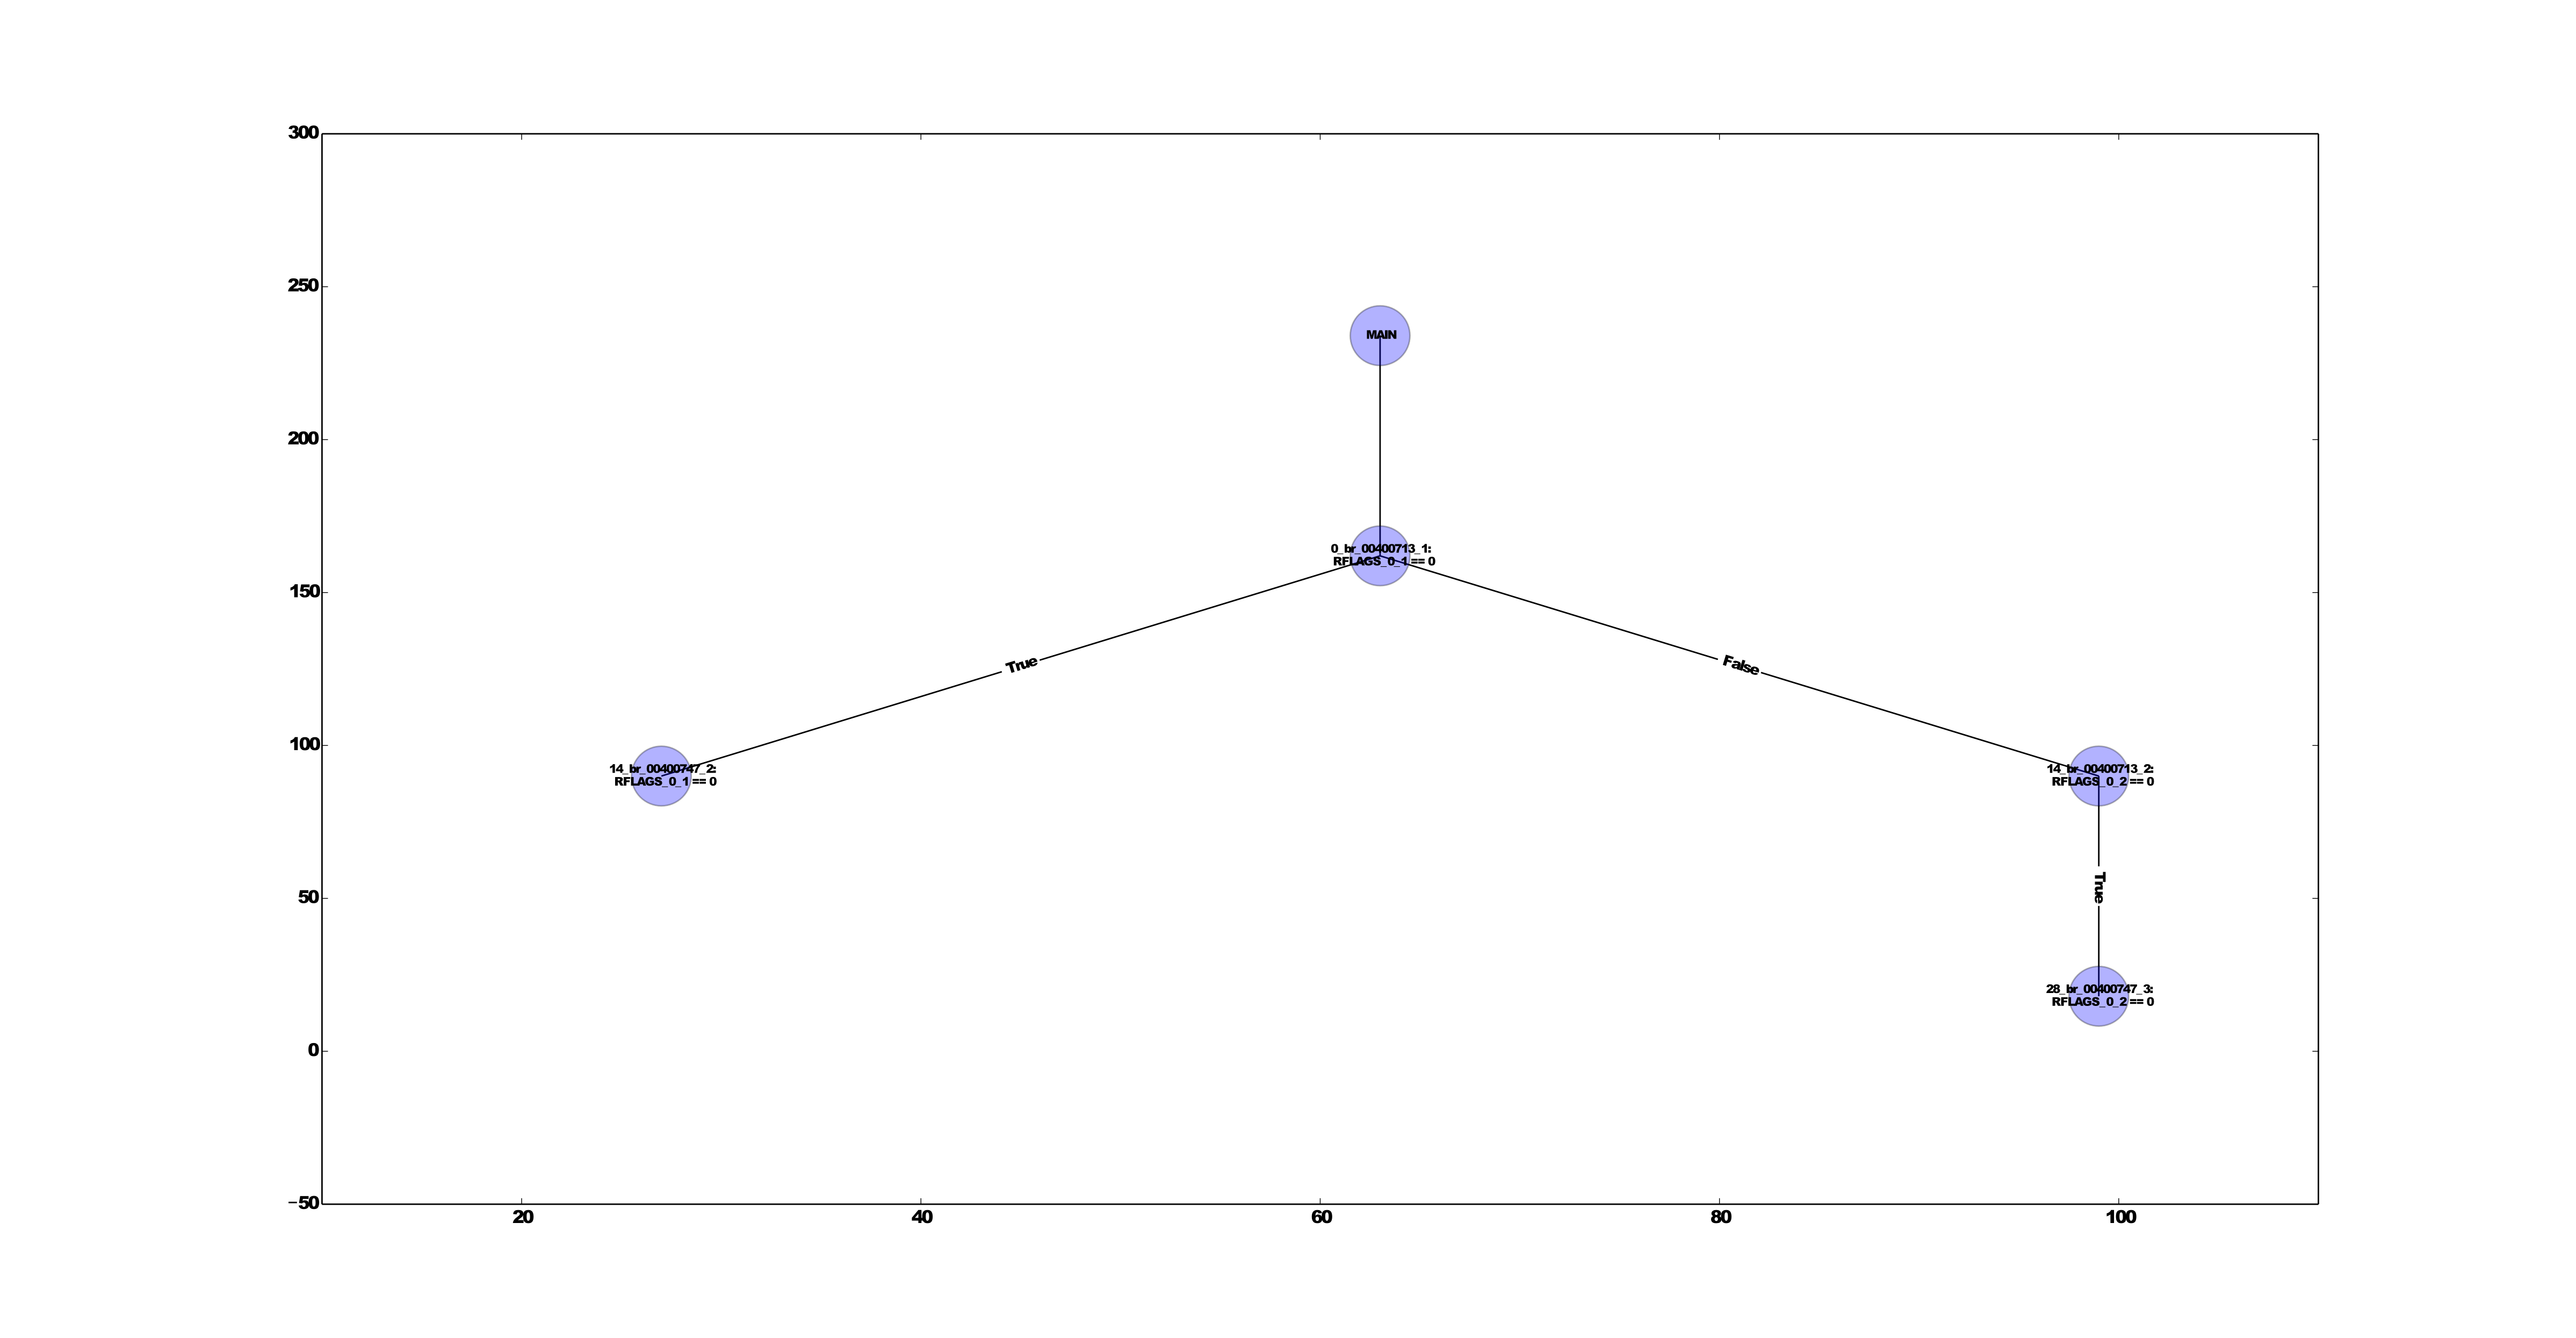
\includegraphics[width=0.45\textwidth]{graphs/2_1}\\\hline
   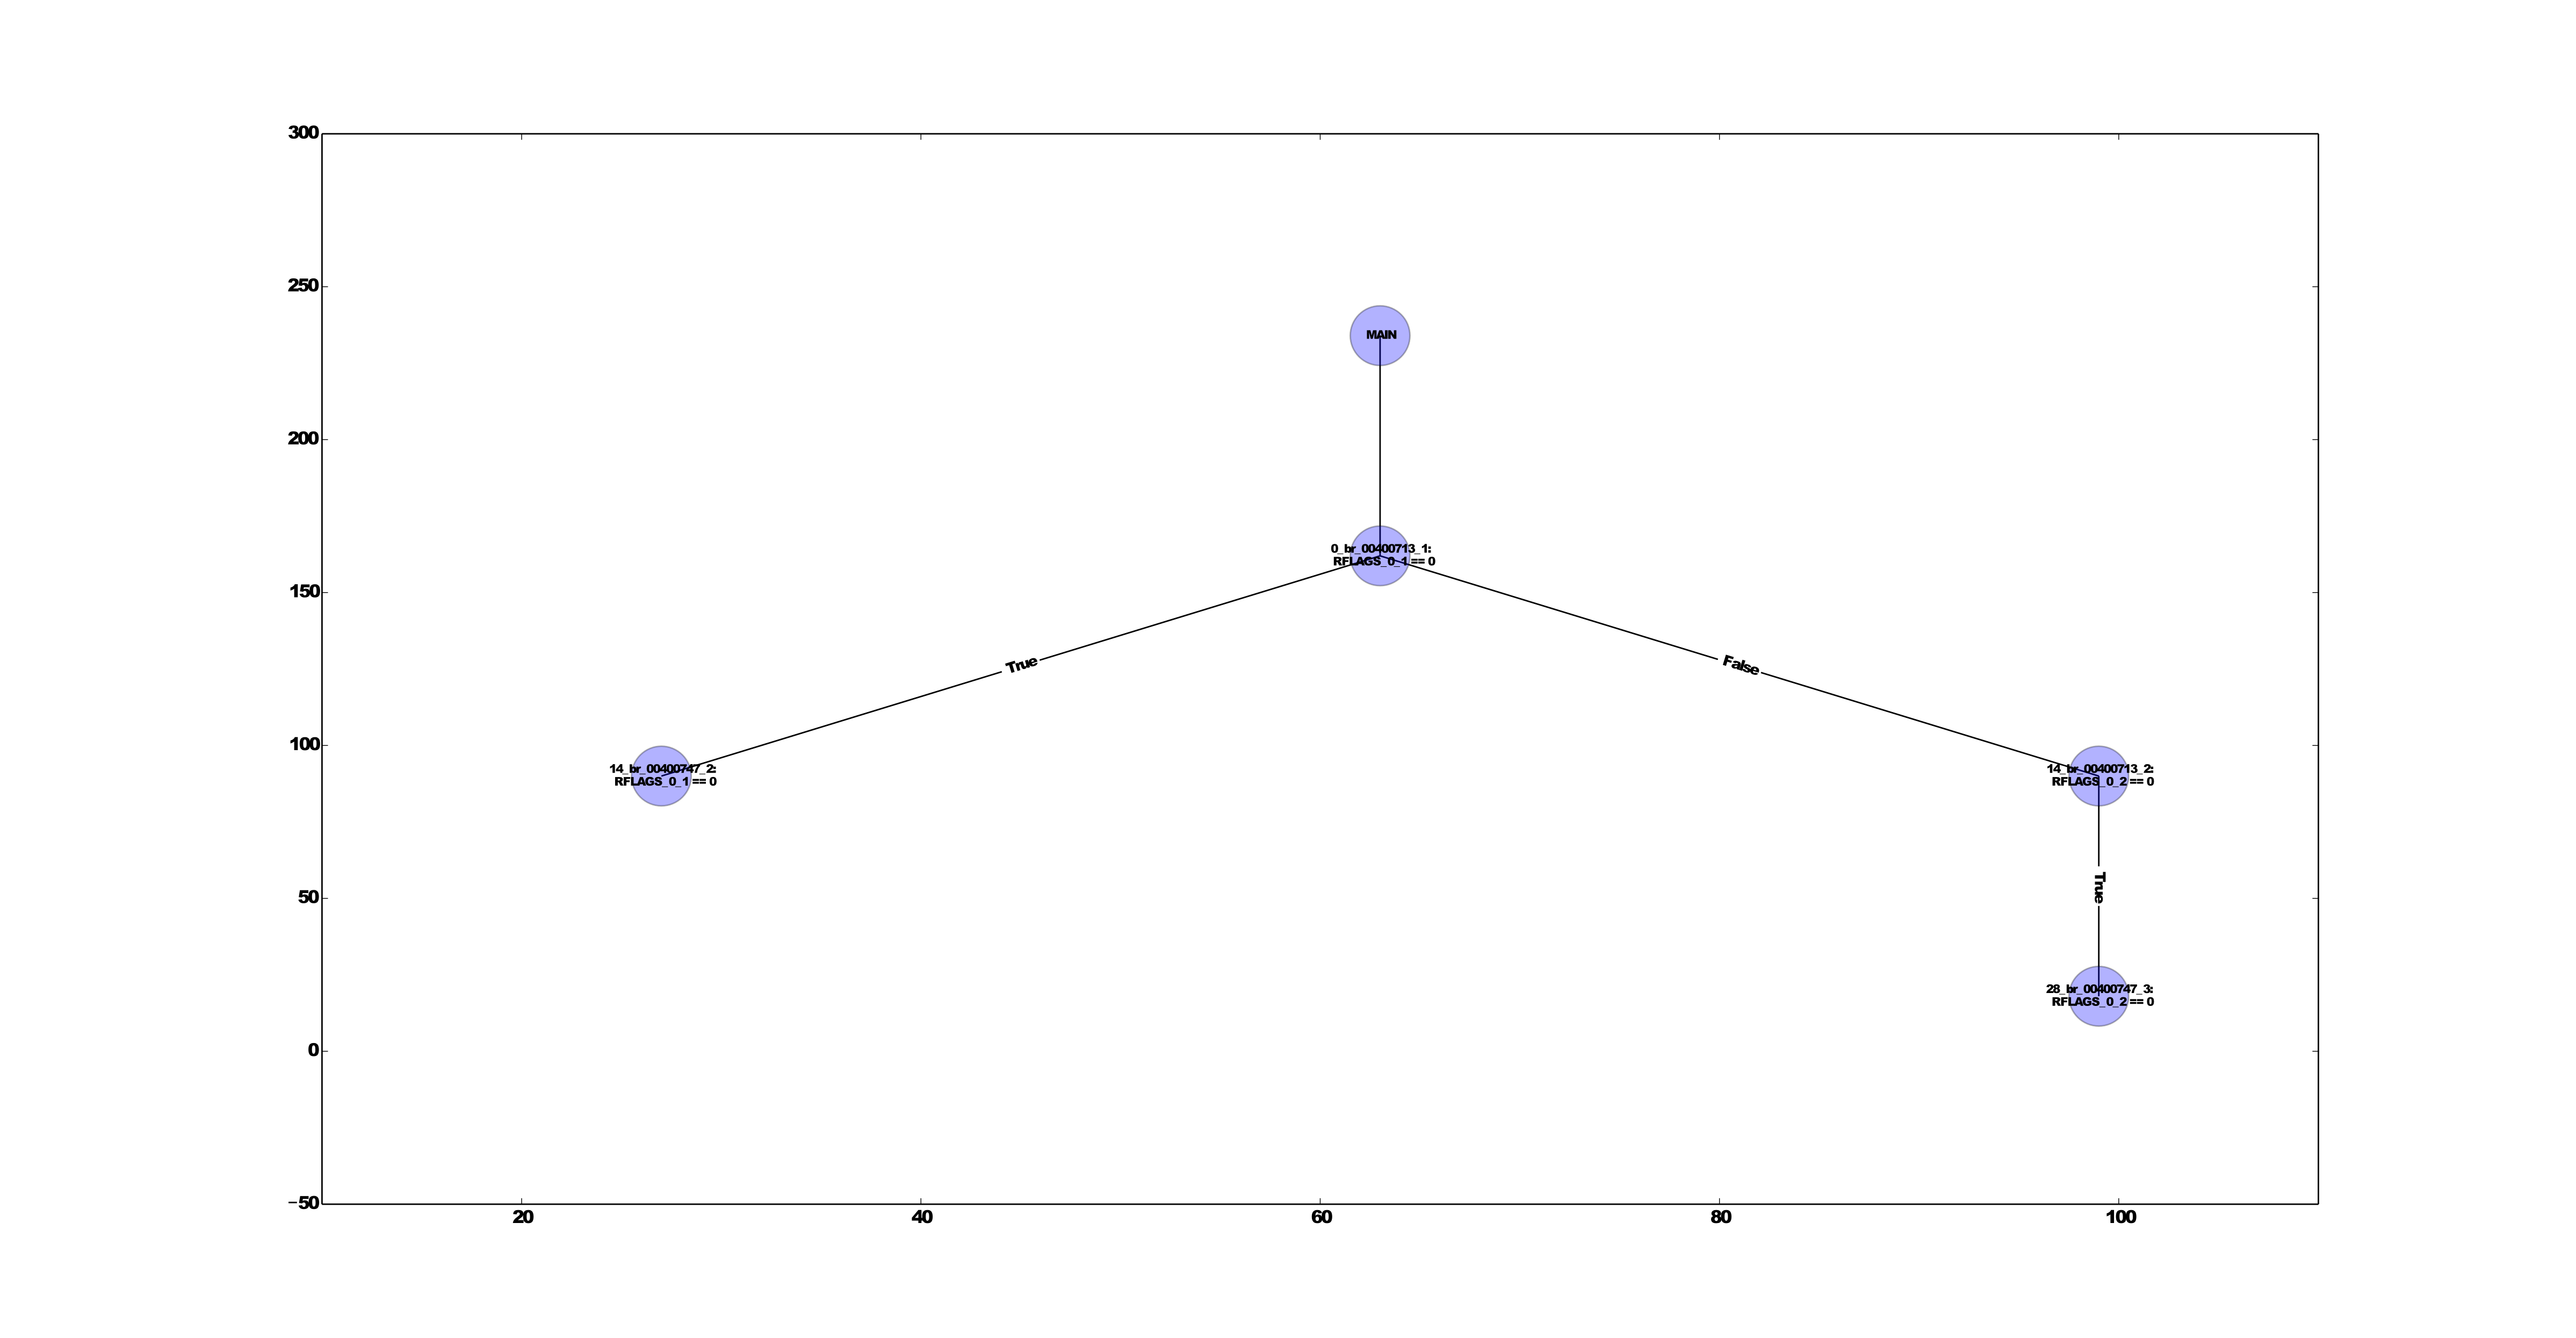
\includegraphics[width=0.45\textwidth]{graphs/2_2}
   &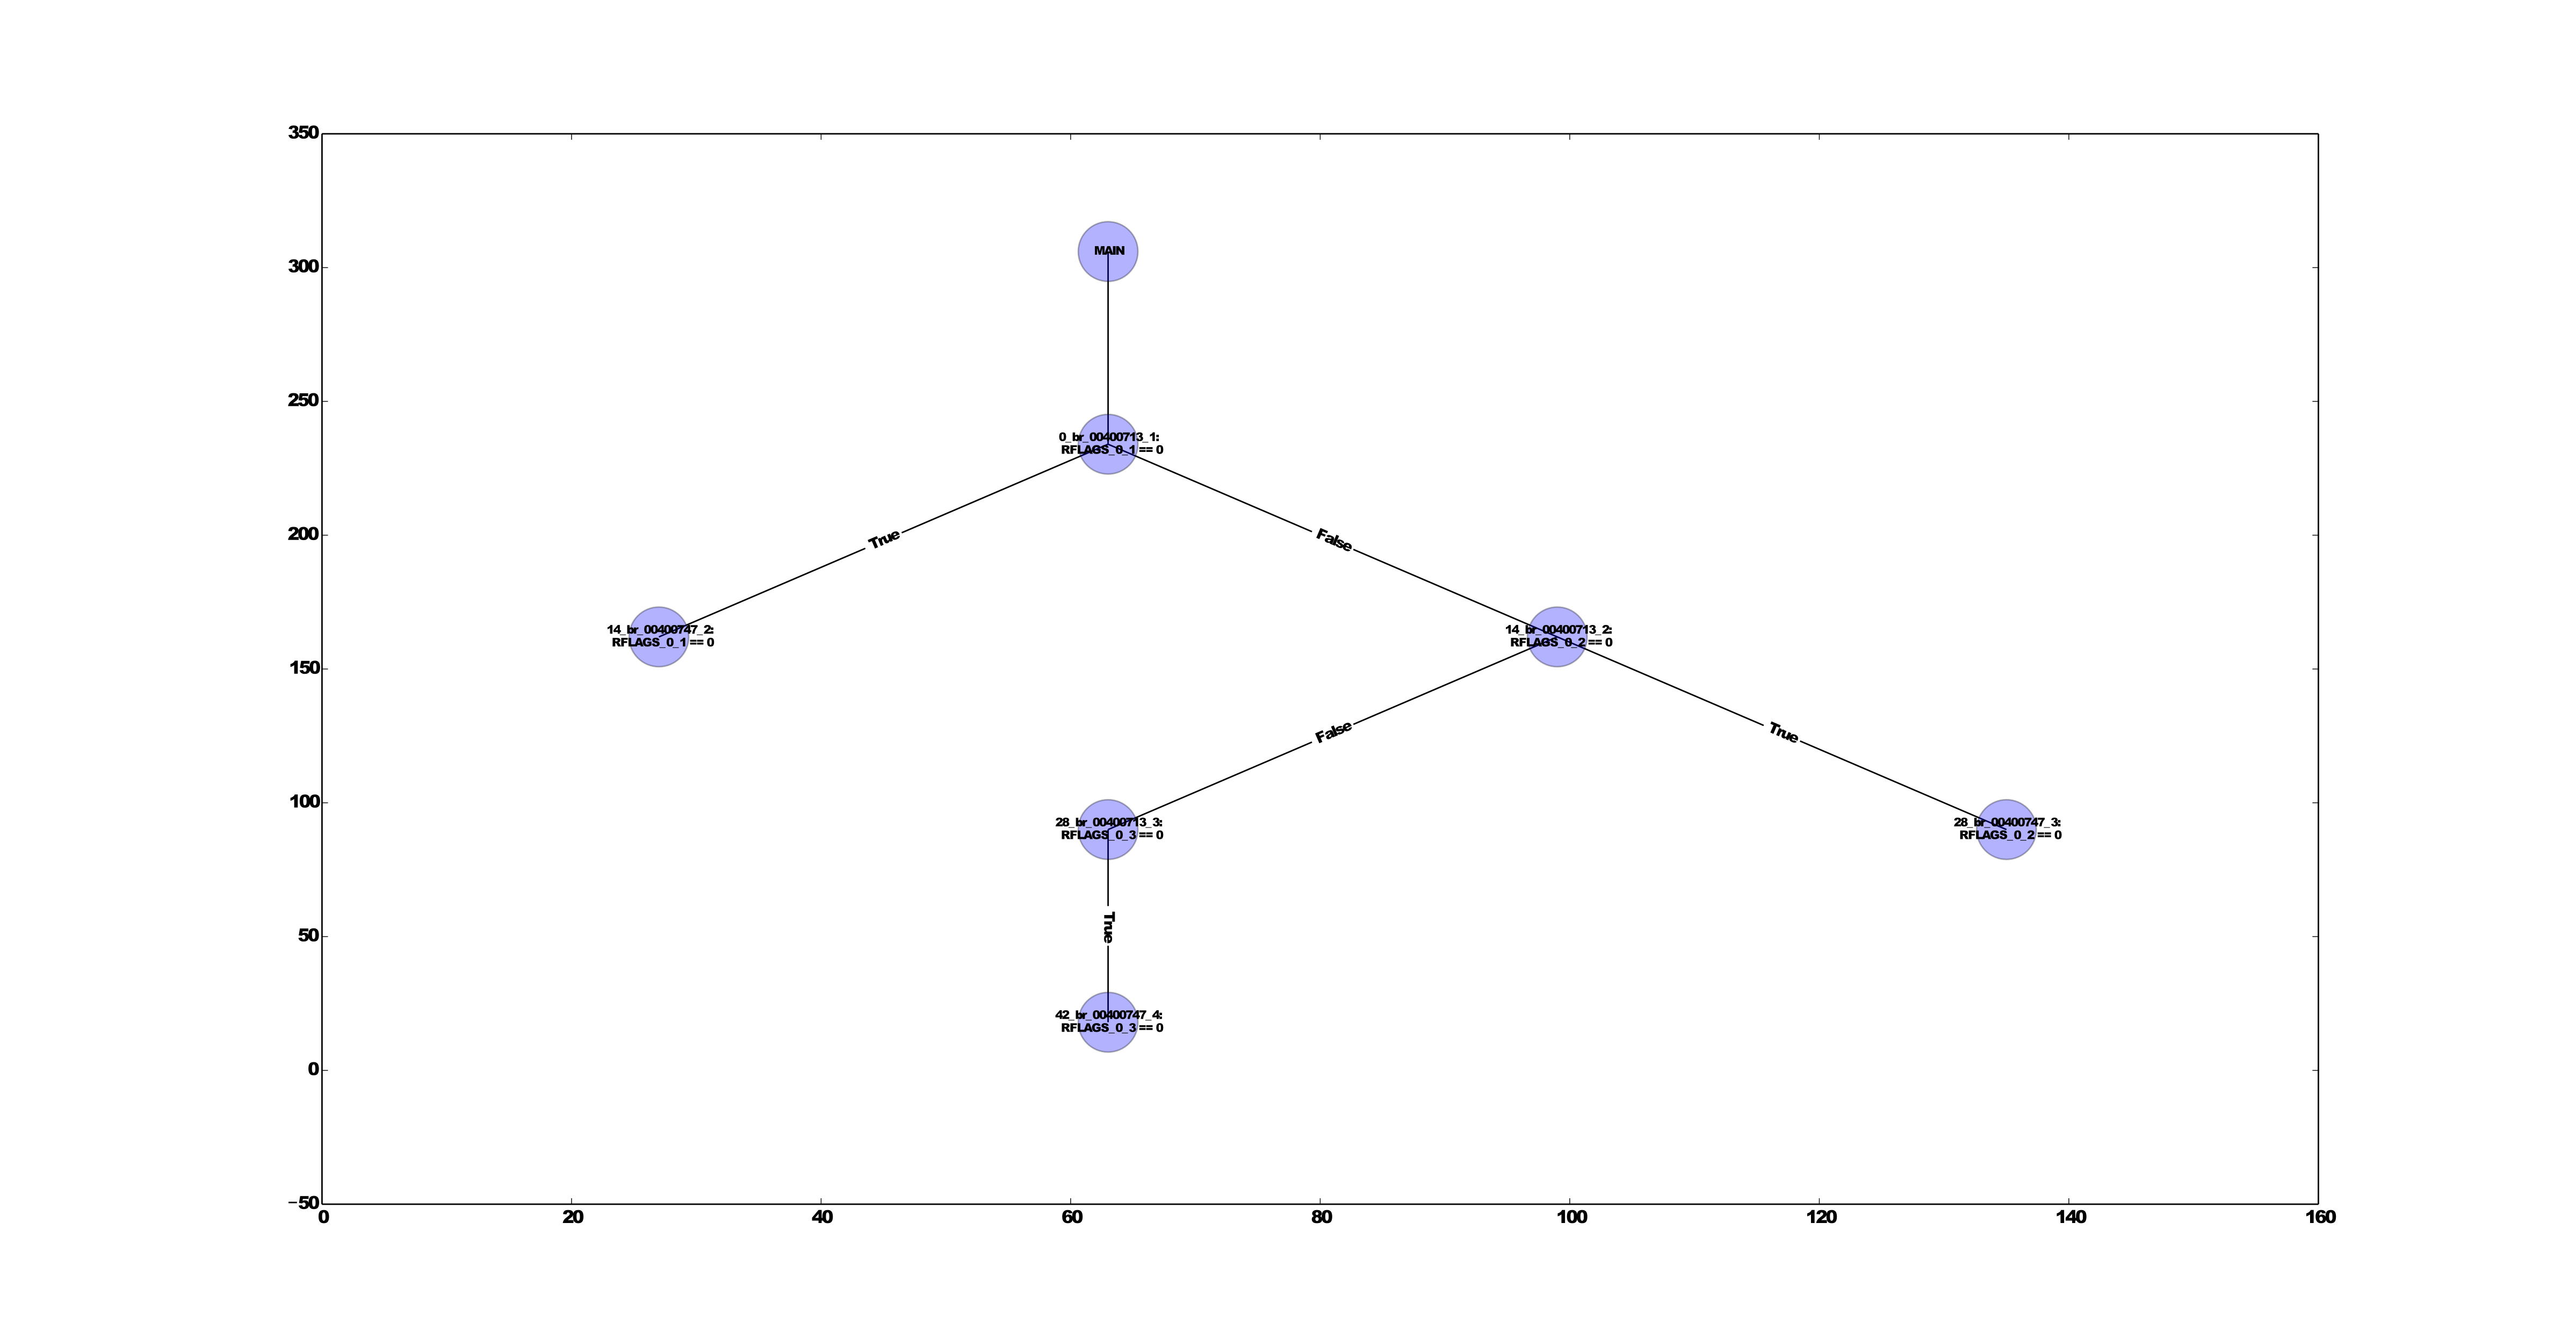
\includegraphics[width=0.45\textwidth]{graphs/2_3}\\\hline
   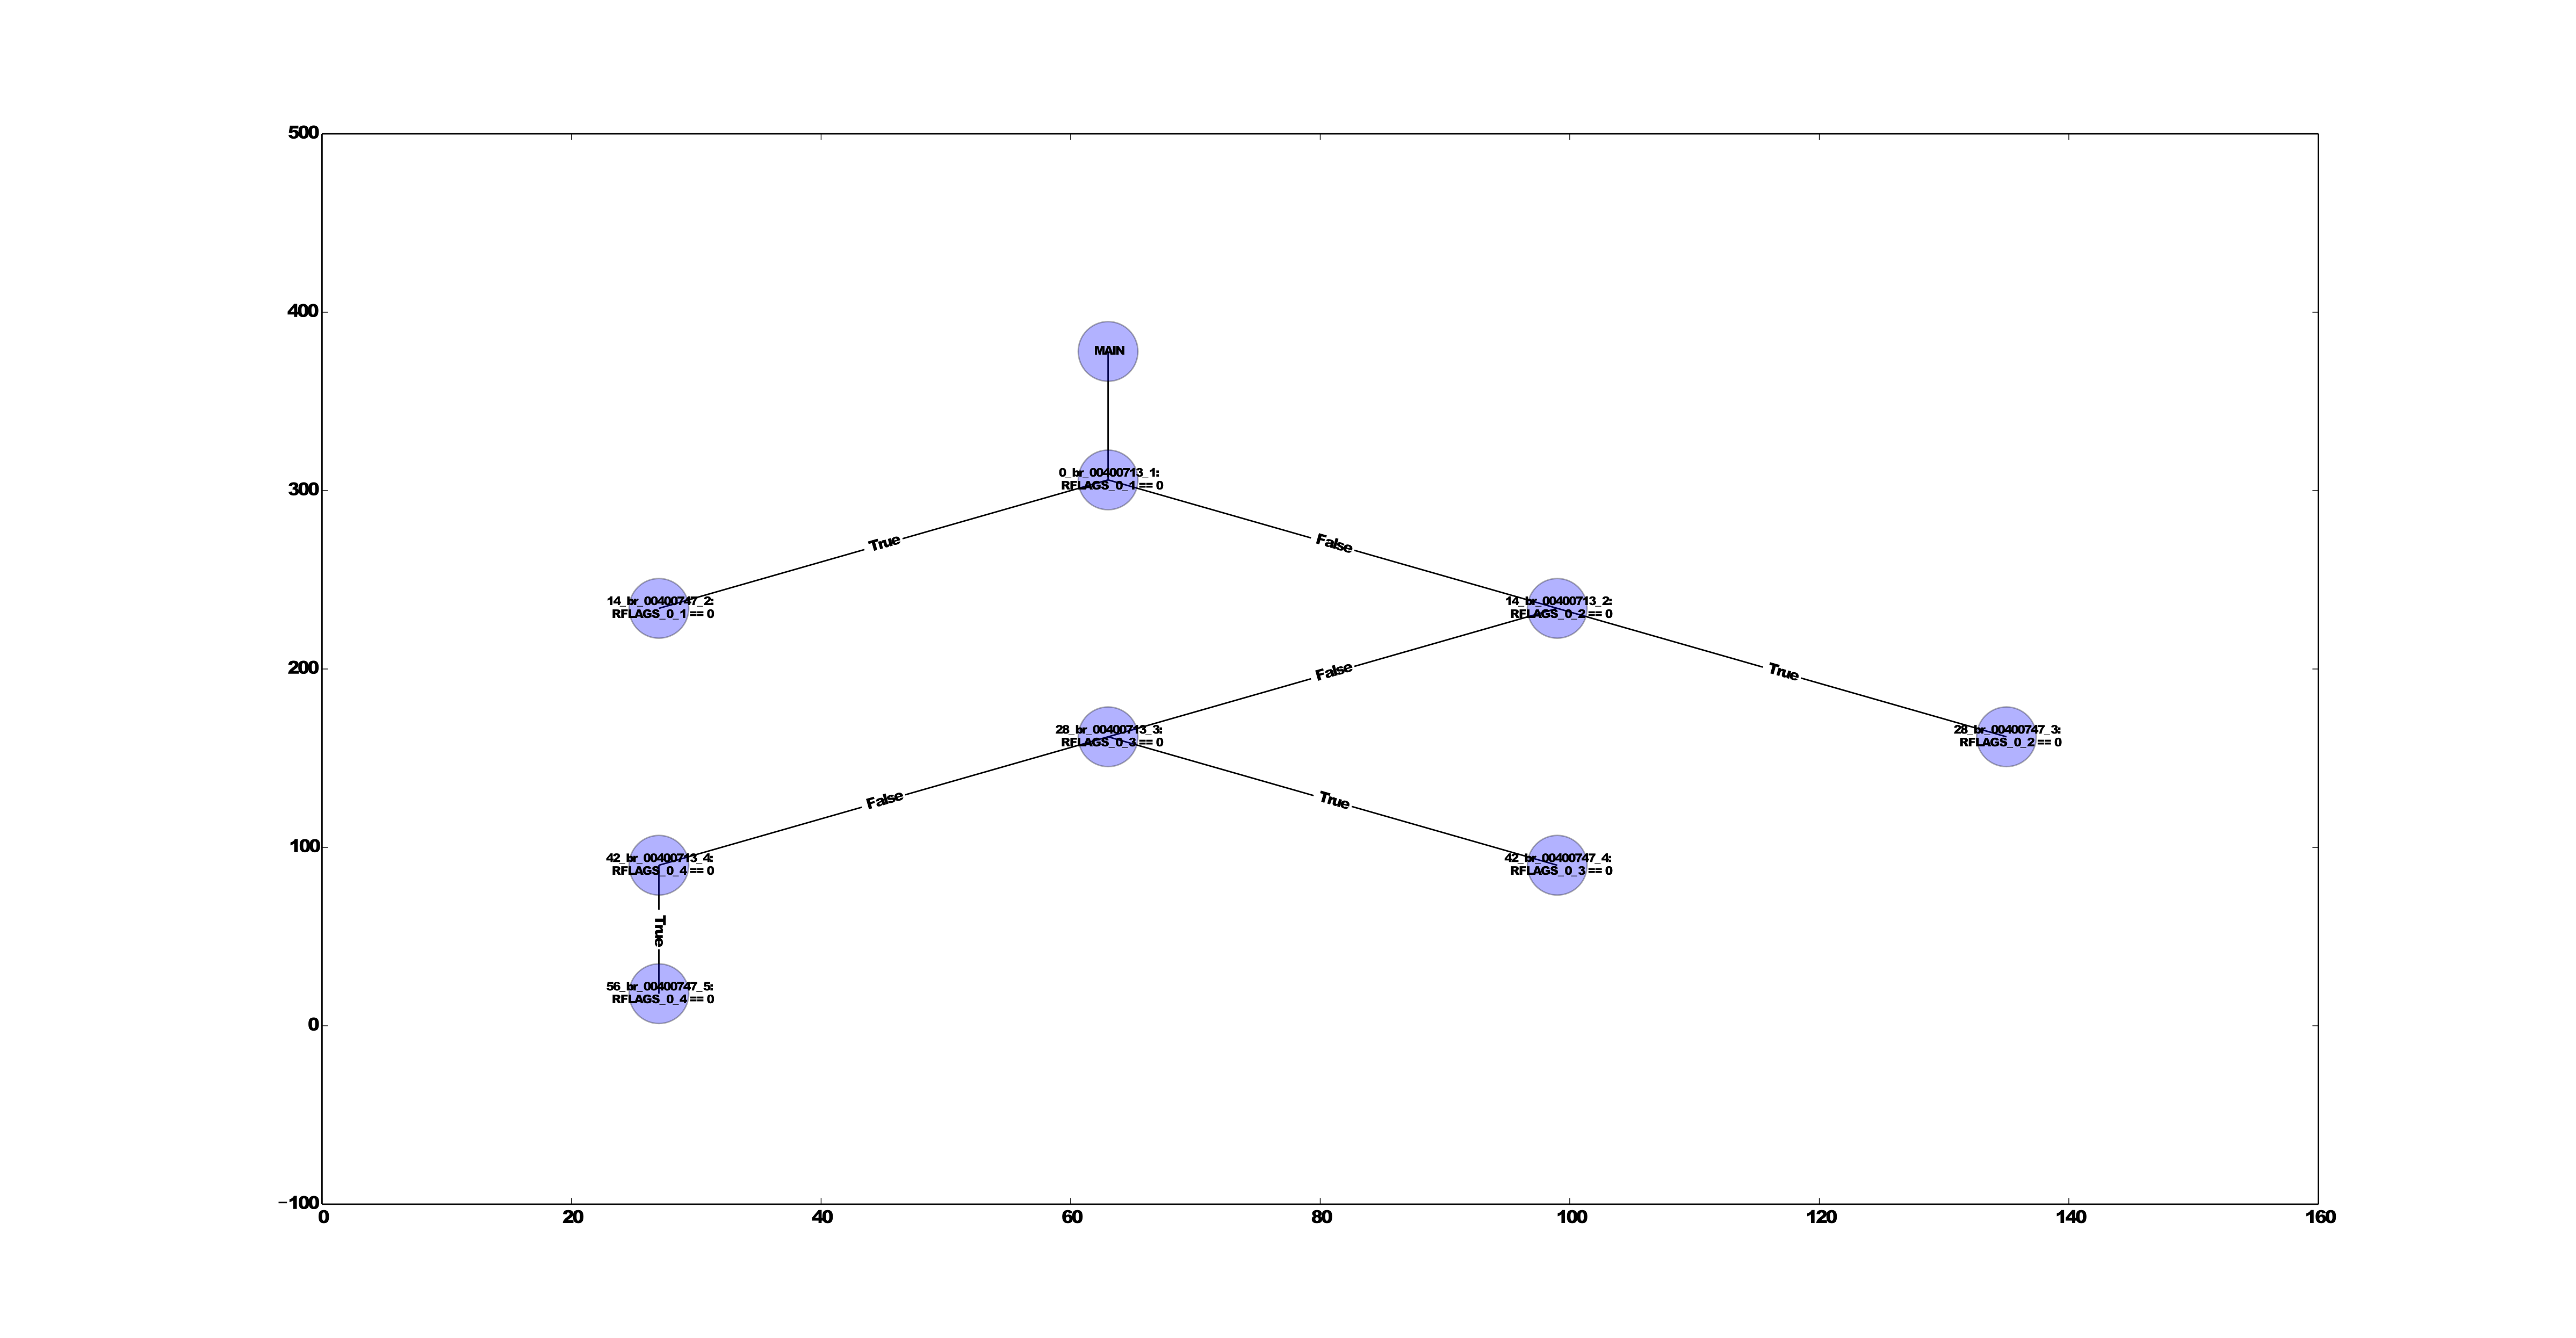
\includegraphics[width=0.45\textwidth]{graphs/2_4}
   &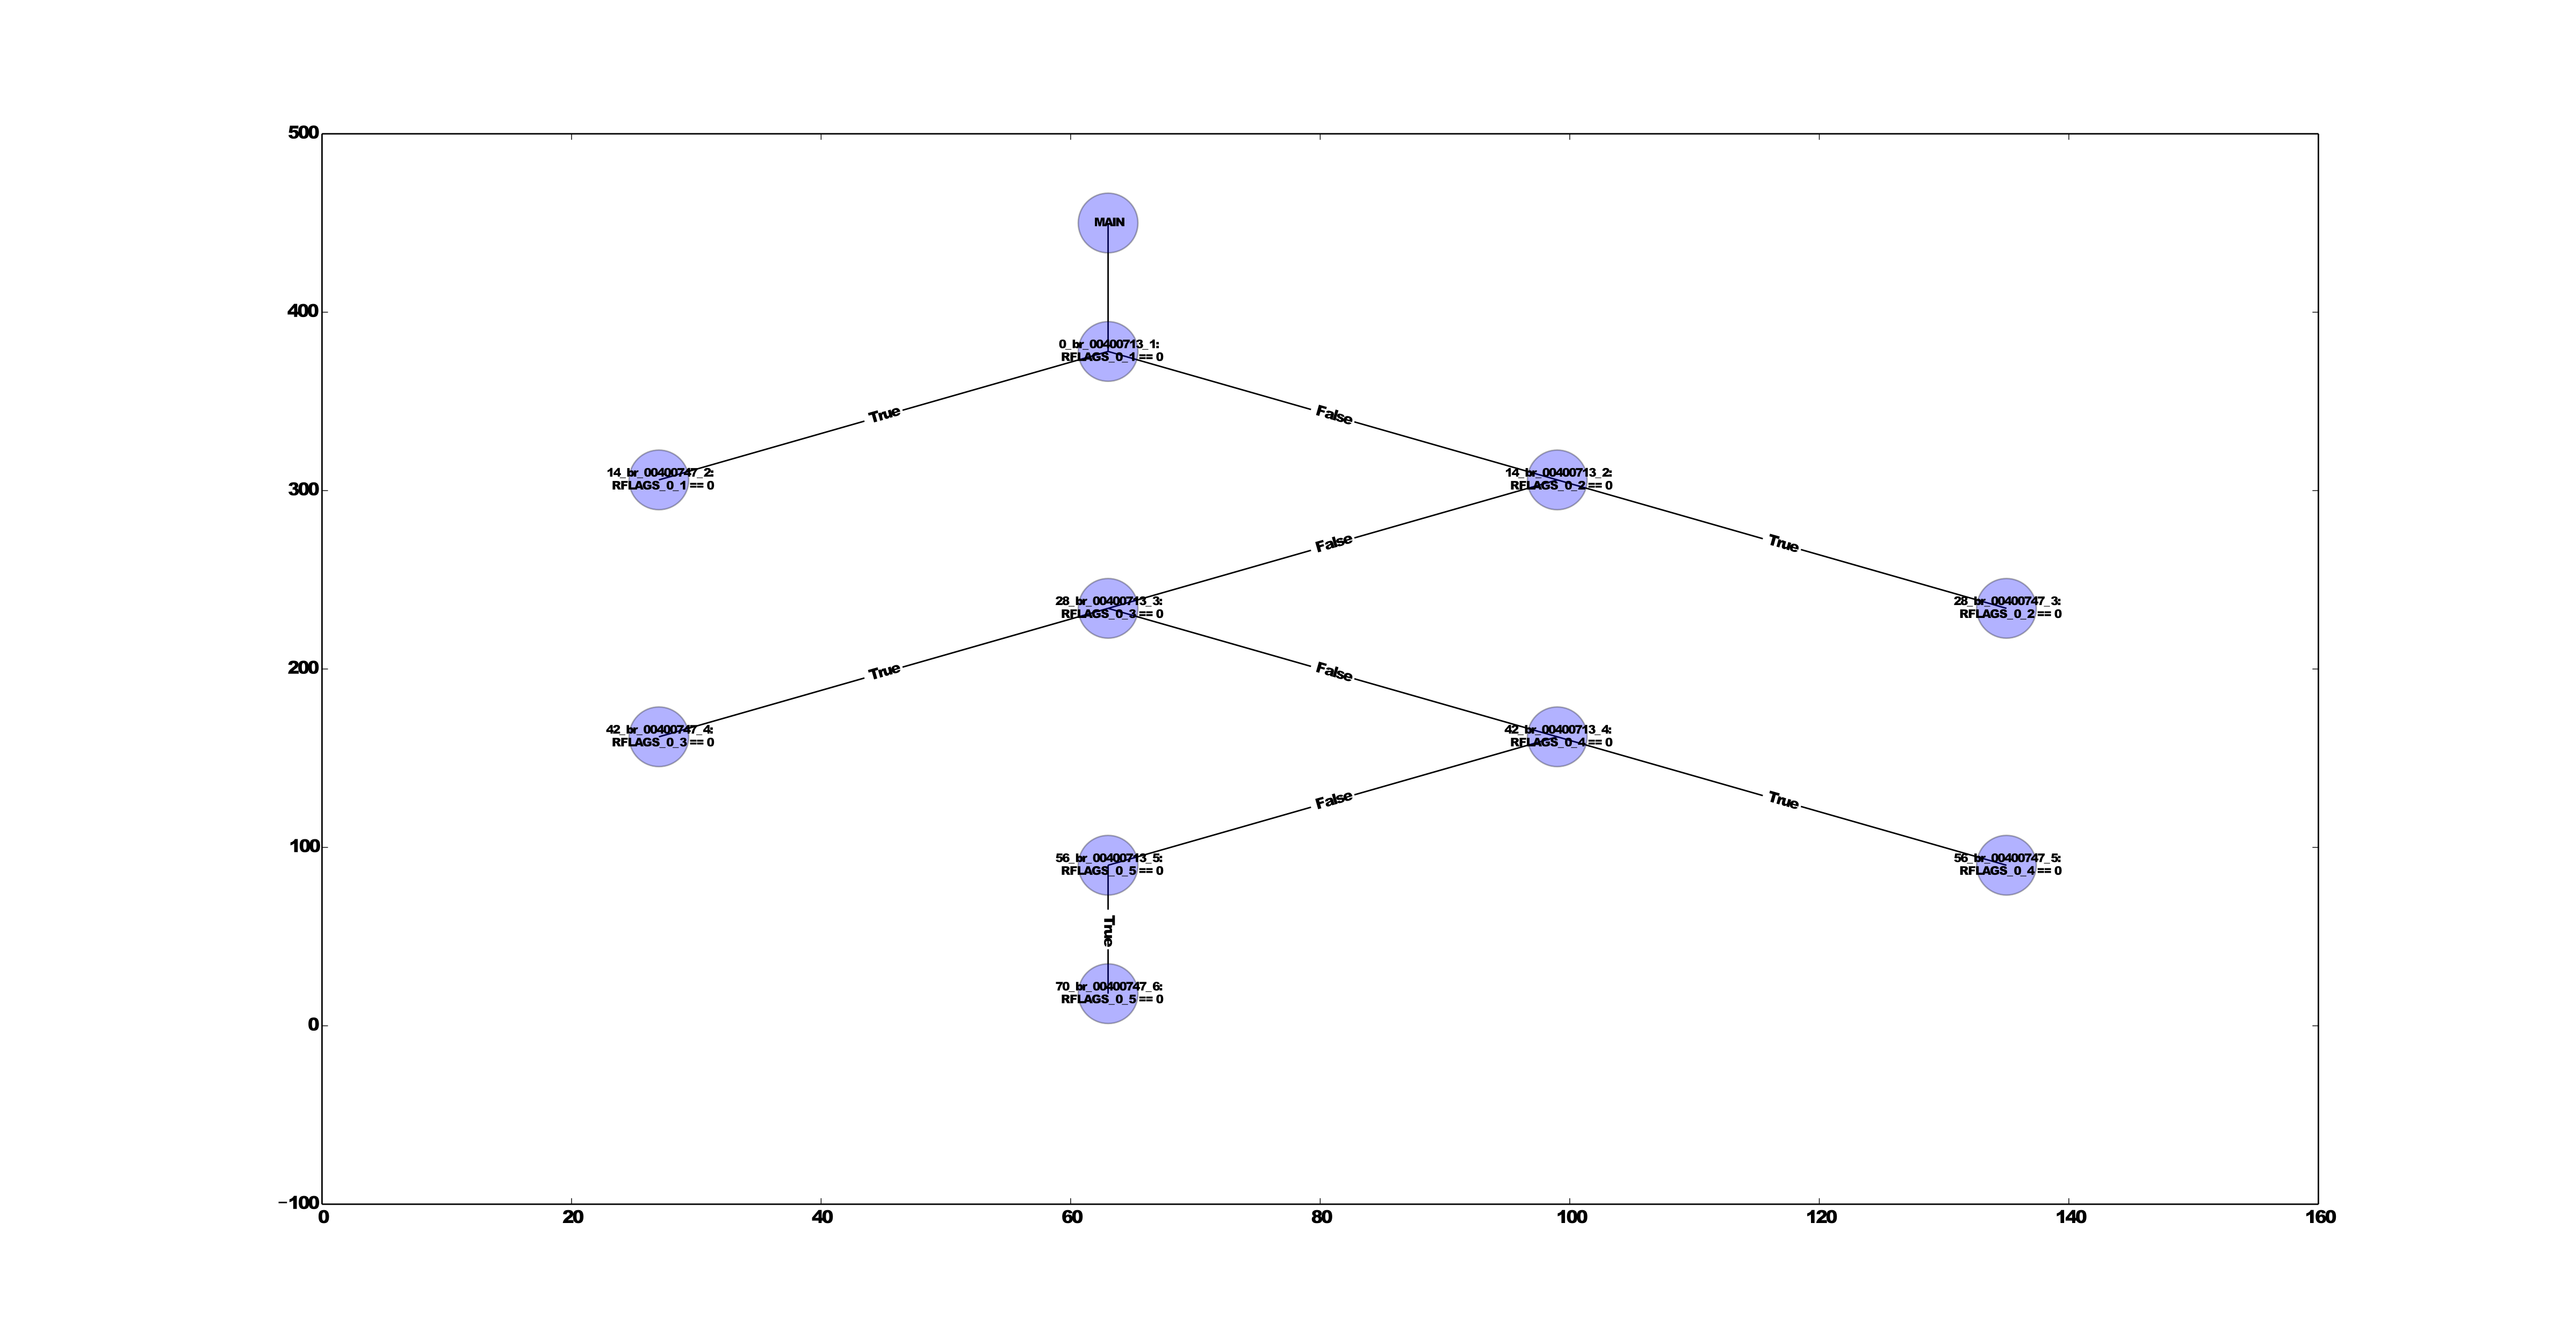
\includegraphics[width=0.45\textwidth]{graphs/2_5}\\\hline
   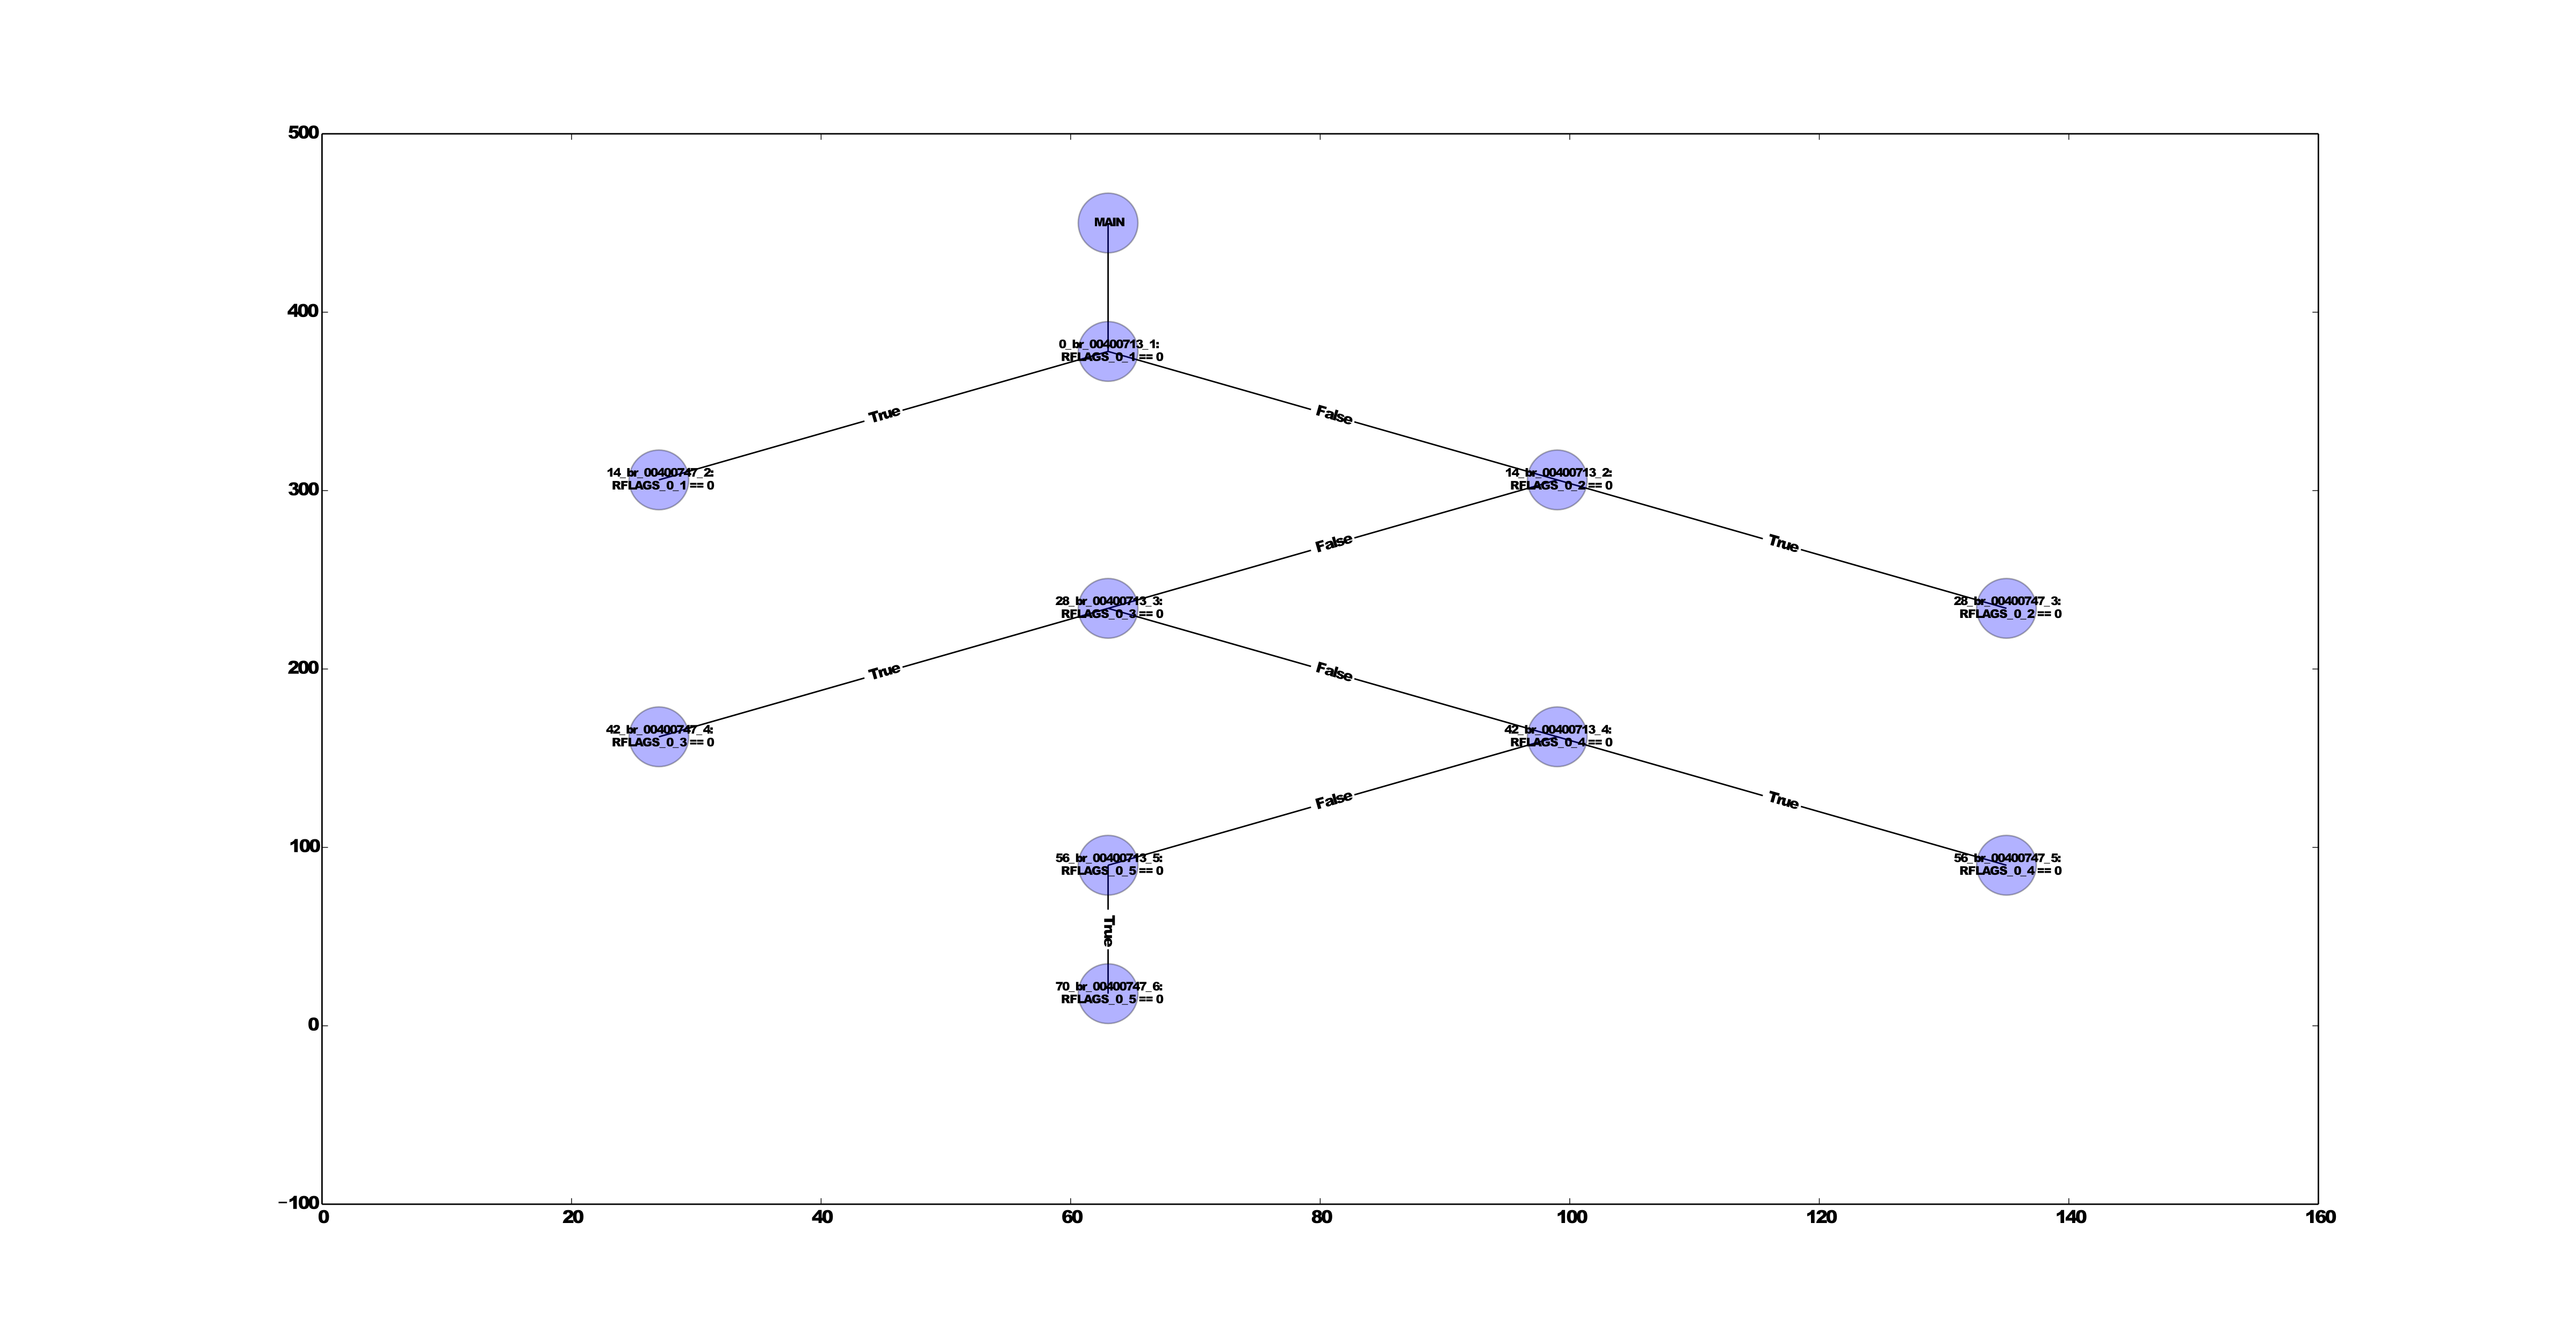
\includegraphics[width=0.45\textwidth]{graphs/2_6}
   &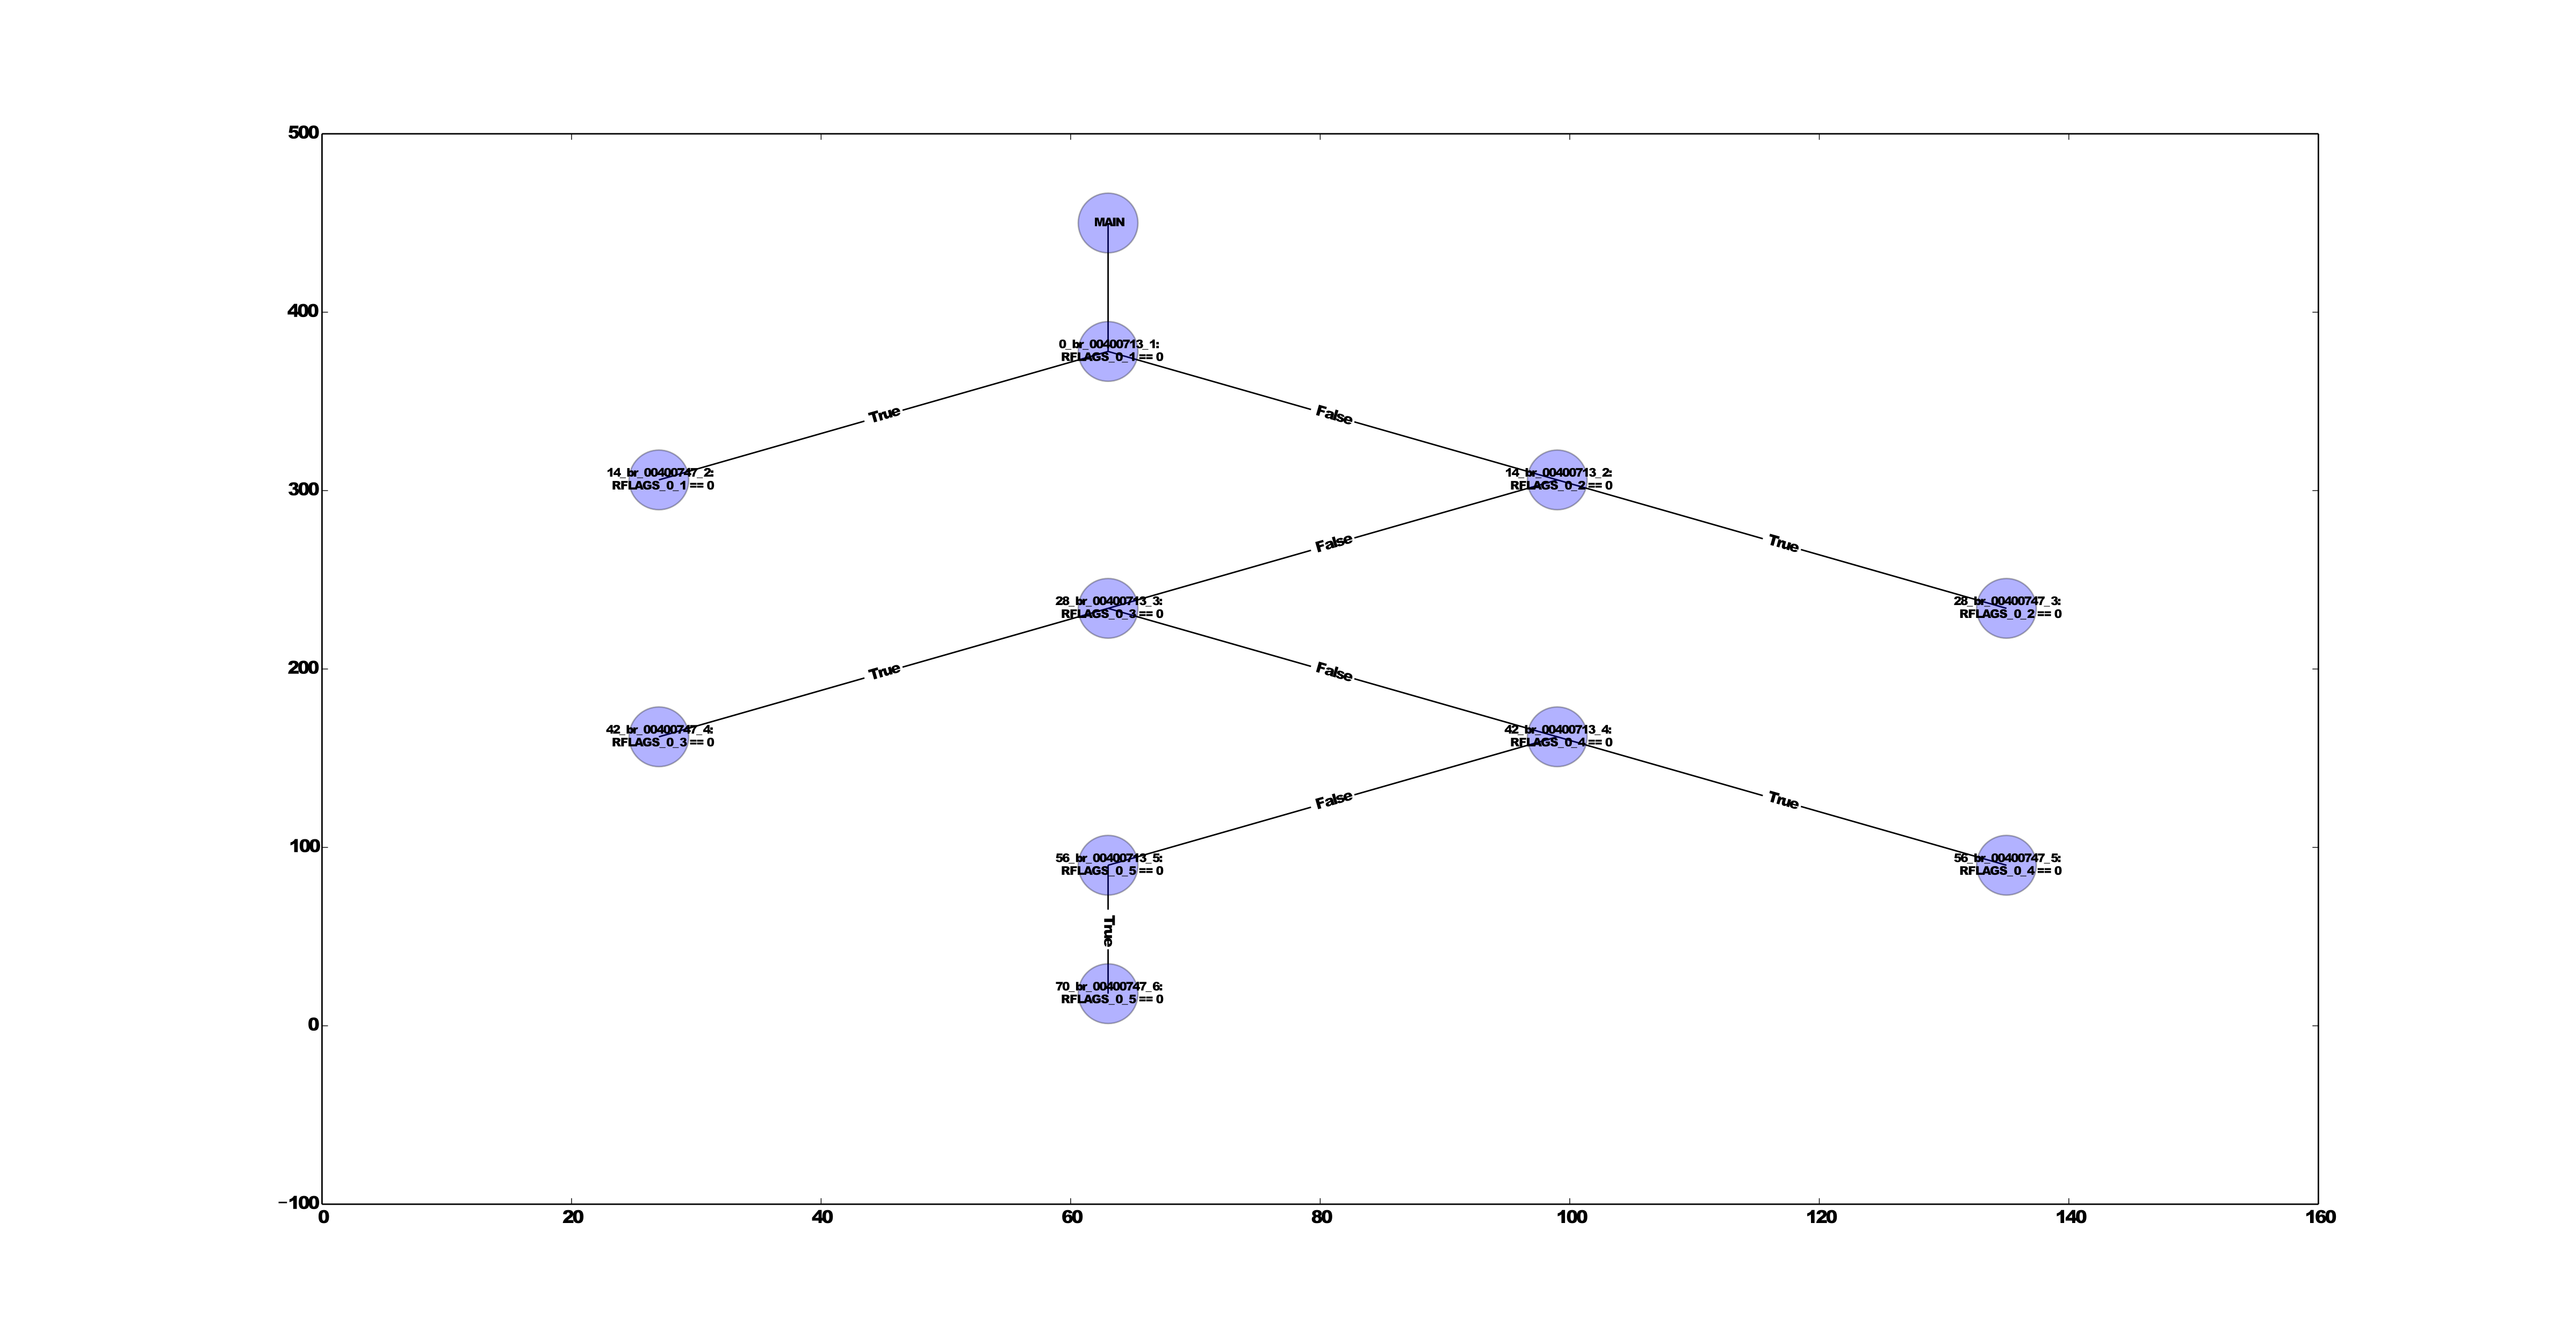
\includegraphics[width=0.45\textwidth]{graphs/2_7}\\\hline
 \end{tabular}
 \caption{Example Execution Graphs for test2}
 \label{figure:examplegraphs2}
\end{figure}
